\ifdefined\pdfinfoomitdate\pdfinfoomitdate=1\fi
\ifdefined\pdftrailerid\pdftrailerid{}\fi
\documentclass[11pt]{article}
\usepackage[T1]{fontenc}
\usepackage{lmodern}
\usepackage[margin=1.05in]{geometry}
\usepackage{microtype}
\usepackage{amsmath,amssymb,amsthm,mathtools}
\usepackage{enumitem,booktabs}
\usepackage{xcolor}
\usepackage{xurl}
\usepackage{tikz}
\usetikzlibrary{arrows.meta,positioning,calc,fit,backgrounds}
\usepackage[colorlinks=true,linkcolor=blue!45!black,citecolor=blue!45!black,urlcolor=blue!45!black]{hyperref}
\hypersetup{pdftitle={Critical slowing down in the Sherrington--Kirkpatrick model},pdfauthor={OpenAI}}
\pdfgentounicode=1
\pdfglyphtounicode{parenleftbig}{0028}
\pdfglyphtounicode{parenleftBig}{0028}
\pdfglyphtounicode{parenleftbigg}{0028}
\pdfglyphtounicode{parenleftBigg}{0028}
\pdfglyphtounicode{parenrightbig}{0029}
\pdfglyphtounicode{parenrightBig}{0029}
\pdfglyphtounicode{parenrightbigg}{0029}
\pdfglyphtounicode{parenrightBigg}{0029}
\pdfglyphtounicode{bracketleftbig}{005B}
\pdfglyphtounicode{bracketleftBig}{005B}
\pdfglyphtounicode{bracketleftbigg}{005B}
\pdfglyphtounicode{bracketleftBigg}{005B}
\pdfglyphtounicode{bracketrightbig}{005D}
\pdfglyphtounicode{bracketrightBig}{005D}
\pdfglyphtounicode{bracketrightbigg}{005D}
\pdfglyphtounicode{bracketrightBigg}{005D}
\pdfglyphtounicode{floorleftbig}{230A}
\pdfglyphtounicode{floorleftBig}{230A}
\pdfglyphtounicode{floorleftbigg}{230A}
\pdfglyphtounicode{floorleftBigg}{230A}
\pdfglyphtounicode{floorrightbig}{230B}
\pdfglyphtounicode{floorrightBig}{230B}
\pdfglyphtounicode{floorrightbigg}{230B}
\pdfglyphtounicode{floorrightBigg}{230B}
\pdfglyphtounicode{ceilingleftbig}{2308}
\pdfglyphtounicode{ceilingleftBig}{2308}
\pdfglyphtounicode{ceilingleftbigg}{2308}
\pdfglyphtounicode{ceilingleftBigg}{2308}
\pdfglyphtounicode{ceilingrightbig}{2309}
\pdfglyphtounicode{ceilingrightBig}{2309}
\pdfglyphtounicode{ceilingrightbigg}{2309}
\pdfglyphtounicode{ceilingrightBigg}{2309}
\pdfglyphtounicode{braceleftbig}{007B}
\pdfglyphtounicode{braceleftBig}{007B}
\pdfglyphtounicode{braceleftbigg}{007B}
\pdfglyphtounicode{braceleftBigg}{007B}
\pdfglyphtounicode{bracerightbig}{007D}
\pdfglyphtounicode{bracerightBig}{007D}
\pdfglyphtounicode{bracerightbigg}{007D}
\pdfglyphtounicode{bracerightBigg}{007D}
\pdfglyphtounicode{angbracketleftbig}{27E8}
\pdfglyphtounicode{angbracketleftBig}{27E8}
\pdfglyphtounicode{angbracketleftbigg}{27E8}
\pdfglyphtounicode{angbracketleftBigg}{27E8}
\pdfglyphtounicode{angbracketrightbig}{27E9}
\pdfglyphtounicode{angbracketrightBig}{27E9}
\pdfglyphtounicode{angbracketrightbigg}{27E9}
\pdfglyphtounicode{angbracketrightBigg}{27E9}
\newcommand{\R}{\mathbb R}
\newcommand{\N}{\mathbb N}
\newcommand{\E}{\mathbb E}
\newcommand{\Prob}{\mathbb P}
\newtheorem{theorem}{Theorem}[section]
\newtheorem{lemma}[theorem]{Lemma}
\newtheorem{proposition}[theorem]{Proposition}
\newtheorem{corollary}[theorem]{Corollary}
\theoremstyle{definition}
\newtheorem{definition}[theorem]{Definition}
\theoremstyle{remark}
\newtheorem{remark}[theorem]{Remark}
\numberwithin{equation}{section}
\setlength{\emergencystretch}{1.5em}
\setlist[enumerate]{leftmargin=*,itemsep=3pt,topsep=5pt}
\setlist[itemize]{leftmargin=*,itemsep=3pt,topsep=5pt}
\DeclareMathOperator{\Var}{Var}
\DeclareMathOperator{\Cov}{Cov}
\DeclareMathOperator{\diag}{diag}
\DeclareMathOperator{\sech}{sech}
\DeclareMathOperator{\Tr}{Tr}
\DeclareMathOperator{\osc}{osc}
\newcommand{\TV}{\mathrm{TV}}
\title{Critical slowing down in the\\Sherrington--Kirkpatrick model}
\author{OpenAI}
\date{September 24, 2026}
\begin{document}
\maketitle
\begin{abstract}
At the critical inverse temperature $\beta=1$, we prove slow mixing for zero-field Gaussian Sherrington--Kirkpatrick heat-bath dynamics from typical equilibrium configurations held fixed as initial states. For every deterministic sequence $t_n=o(n^{2/3})$ in rate-one-per-site time, the Gibbs mass of initial states whose time-$t_n$ total-variation distance from equilibrium exceeds $1/4$ tends to one in probability over the disorder. The same statement holds for every deterministic integer sequence $k_n=o(n^{5/3})$ of uniform-site update attempts.
\end{abstract}
\section{Introduction}\label{sec:introduction}
At the critical temperature of the Sherrington--Kirkpatrick model,
equilibrium fluctuations contain a direction that local spin updates
can change only slowly. We use this fluctuation to prove a total-variation
obstruction for most equilibrium configurations viewed as fixed initial
states. The same static estimates determine the covariance scale and
the relaxation detected by linear observables.

\subsection{The model and main results}
The model introduced by Sherrington and Kirkpatrick \cite{sk1975}
places spins on $\Omega_n=\{-1,1\}^n$ and couples every pair through an
independent Gaussian variable. At inverse temperature $\beta=1$ and zero field,
$W_{ij}\sim N(0,1/n)$ for $i<j$, and
\begin{equation}\label{eq:intro-law}
 \mu_W(x)\propto
 \exp\!\left(\sum_{i<j}W_{ij}x_ix_j\right),
 \qquad x\in\{-1,1\}^n.
\end{equation}
Here $\beta=1$ marks the large-$n$ equilibrium spin-glass transition
\cite[Section~1, after Equation~(1.4)]{duHuang2026FreeEnergy}. The overlap
$n^{-1}x^Ty$ of two independent equilibrium replicas has scale $n^{-1/3}$
at criticality, compared with its Gaussian $n^{-1/2}$ scale at each fixed
$\beta<1$ \cite[Equation~(1.1) and Theorem~1.1]{duHuang2026Overlap}.
A heat-bath update resamples one spin from its conditional law under
$\mu_W$. We use two clocks: in continuous time each site has an independent
rate-one clock; in discrete time each step attempts one update at a
uniformly chosen site. An attempt may leave the spin unchanged.

For fixed disorder and initial configuration $x$, let
$d_t^{\rm ct}(W,x)$ and $d_k^{\rm dt}(W,x)$ denote the total-variation
distances of the corresponding transition laws from $\mu_W$.
Section~\ref{sec:model} gives the operators and conventions in detail.
Our first result concerns an equilibrium configuration after its realized
value has been fixed as the initial state. All probability limits in the
main results are over the original off-diagonal Gaussian disorder.

\begin{theorem}[Realized equilibrium initial states]\label{thm:gibbs-start}
For every deterministic sequence $t_n\ge0$ with $t_n=o(n^{2/3})$,
\[
 \mu_W\{x:d_{t_n}^{\rm ct}(W,x)>1/4\}
 \xrightarrow{\Prob}1.
\]
For every deterministic integer sequence $k_n\ge0$ with $k_n=o(n^{5/3})$,
\[
 \mu_W\{x:d_{k_n}^{\rm dt}(W,x)>1/4\}
 \xrightarrow{\Prob}1.
\]
The convergence is in probability over the disorder.
\end{theorem}

The theorem tests each realized start separately: averaging its transition
law over the equilibrium initial configuration would give the stationary
law $\mu_W$. It also treats each prescribed deterministic time sequence
separately; the set of slowly mixing starts may depend on that sequence.

To state the static conclusion, set $\Sigma=\Cov_{\mu_W}(x)$ and define
the unscaled conditional-variance form
\[
 \mathcal D_{\mu_W}(f)
 =\sum_{i=1}^n\mu_W[\Var(f\mid x_{-i})].
\]
Here $x_{-i}$ comprises every spin except $i$. This is the Dirichlet
form for the rate-one-per-site clock. The largest inverse Rayleigh quotient
among linear functions is
\[
 \mathcal R_{\rm lin}(\mu_W)
 =\sup_{a\in\R^n\setminus\{0\}}
   \frac{\Var_{\mu_W}(a^Tx)}{\mathcal D_{\mu_W}(a^Tx)}.
\]

\begin{theorem}[Covariance and linear tests]\label{thm:linear-scale}
For every positive deterministic sequence $M_n\to\infty$, with probability tending to one both $\|\Sigma\|$ and $\mathcal R_{\rm lin}(\mu_W)$ belong to
\[
 \left[\frac{n^{2/3}}{M_n},\ M_n n^{2/3}\right].
\]
\end{theorem}

The factor $M_n$ may diverge more slowly than any prescribed power or
logarithm. Because the quotient here ranges only over linear functions,
its upper bound does not control the full inverse spectral gap.

For comparison with customary worst-start mixing, let $t_{\rm mix}$ and
$k_{\rm mix}$ be the first continuous time and the first integer step,
respectively, at which every initial configuration has distance at most
$1/4$. Theorem~\ref{thm:gibbs-start} gives the lower bounds below. An
independent comparison with one fixed high-temperature model gives the
subexponential upper bounds.

\begin{theorem}[Critical mixing bounds]\label{thm:mixing}
For every fixed $\epsilon>0$,
\begin{align}
 \Prob\!\left\{n^{2/3-\epsilon}\le t_{\rm mix}
                   \le e^{\epsilon n}\right\}&\longrightarrow1,
       \label{eq:continuous-main}\\
 \Prob\!\left\{n^{5/3-\epsilon}\le k_{\rm mix}
                   \le e^{\epsilon n}\right\}&\longrightarrow1.
       \label{eq:discrete-main}
\end{align}
\end{theorem}

\subsection{Historical and mathematical context}
Critical spin-glass relaxation has been studied through several models
and convergence criteria. Kirkpatrick and Sherrington
\cite{kirkpatrickSherrington1978} investigated Glauber autocorrelations
above the critical temperature using a linearized mean-field treatment.
Sompolinsky and Zippelius developed equations for disorder-averaged
correlation and response \cite{sompolinskyZippelius1981}, and treated
soft-spin Langevin dynamics in \cite{sompolinskyZippelius1982}. For Ising dynamics,
Billoire and Campbell \cite{billoireCampbell2011} numerically examined
equilibrium autocorrelations on an $n^{2/3}$ scale, with time in updates
per spin. These studies concern correlation and response; the present
paper instead tests total variation after each realized equilibrium start.

Our static comparison uses a spherical model, a classical counterpart of
the Ising spin glass. In their thermodynamic analysis, Kosterlitz,
Thouless, and Jones \cite{kosterlitzThoulessJones1976} located its transition
at the spectral edge and identified the top eigenmode as the ordering
direction. Comets
\cite[Equations~(2.1)--(2.2)]{comets1996} gave the fixed-spectrum
Haar-averaging identity relating the two partition functions. Baik and Lee
\cite{baikLee2016} proved Gaussian and Tracy--Widom spherical free-energy
limits at fixed temperatures on the two sides of criticality, and Landon
\cite{landon2022} treated the critical Gaussian limit and the saddle's
$n^{-2/3}$ edge scale. Bhattacharya and Sen \cite{bhattacharyaSen2016}
reduced fixed-spectrum Haar second moments through the two eigenvalues
$1\pm q$, where $q=x^Ty/n$ is the overlap of two vectors of norm $\sqrt n$,
comparing free-energy exponential rates under
high-temperature spectral assumptions.

The critical results of Du and Huang are close predecessors of the static
estimates used here. For the normalized Ising and spherical partition
functions $Z_{\mathrm{Is}}$ and $Z_{\mathrm{sph}}$ built from the same GOE
matrix, their free-energy work
\cite[Theorems~1.4 and~1.6]{duHuang2026FreeEnergy} proves
\[
 \E\!\left[\left(\frac{Z_{\mathrm{Is}}}{Z_{\mathrm{sph}}}-1\right)^2\right]
 =O(n^{-1/3})
\]
and an annealed squared-overlap estimate of order $n^{-2/3}$.
Their subsequent work \cite[Theorem~1.1]{duHuang2026Overlap}
determines the limiting quenched critical overlap distribution.

Those results also give an alternative route to the static inputs of
this paper. Proposition~4.1 in \cite{duHuang2026Overlap} gives convergence
of the rescaled spectral coefficients, while the proof of Lemma~4.5
identifies the corresponding spherical coordinates. Together with the
fixed-coordinate convergence in the proof of Lemma~4.7,
Equations~(4.24)--(4.26), and the absolutely continuous limiting marginal
in Equation~(2.14), these facts imply
vanishing mass in every deterministic shrinking top-coordinate window.
The restricted Haar first moment and the partition comparison in
\cite[Theorem~1.6]{duHuang2026FreeEnergy} then transfer this estimate to
the cube. The annealed squared-overlap bound also implies, by Markov's inequality, that
$n^{2/3}\E_{\mu_W^{\otimes2}}q(x,y)^2$ is bounded in probability; this is
the overlap input for the covariance upper bound and the cavity argument.
The sign and cavity arguments in Section~\ref{sec:dynamics} give the
additional dynamical and linear-observable deductions.
Our technical sections provide a separate static proof, uniform on
chosen deterministic spectral events, using exact Gaussian conditioning,
a quantitative cubic deficit, and monotone outward overlap bins.

Two further groups of methods enter the proof. The GOE tridiagonal
representation is classical \cite{dumitriuEdelman2002}; our spectral
estimates develop the quadratic-form approach of Ram\'irez, Rider, and
Vir\'ag \cite{ramirezRiderVirag2011} and Ledoux and Rider
\cite{ledouxRider2010}. For the independent upper comparison we use the
fixed-$\beta<1$, zero-field heat-bath Poincar\'e theorem
\cite[Theorem~1.1]{skgapcompanion}. Bauerschmidt and Bodineau
\cite{bauerschmidtBodineau2019} proved a logarithmic Sobolev inequality
with the full spin-flip-gradient form, while Eldan, Koehler, and Zeitouni
\cite{eldanKoehlerZeitouni2022} proved a heat-bath Poincar\'e inequality
for interaction matrices satisfying $0\preceq J\prec I$. After a diagonal shift, their SK applications
reach $\beta<1/4$. More recently, Wang \cite{wang2026SKMixing} proved
worst-start heat-bath mixing to total-variation error $\varepsilon$ in
$O_\beta(n\log(n/\varepsilon))$ attempted updates for fixed $\beta<1/2$,
uniformly over external fields on one
high-probability disorder event. Boban, Li, and Oveis Gharan
\cite{bobanLiOveisGharan2026SK} proved a constant unscaled gap and
zero-field worst-start mixing in $O(n^2)$ attempted updates for $\beta<1/2+\varepsilon_0$
with an absolute $\varepsilon_0>0$, with high probability over the disorder.
The fixed-$\beta<1$ companion input
used here covers the temperatures required by the comparison in
Section~\ref{sec:dynamics}, which fixes $\beta$ before taking $n$ to infinity.

The companion \emph{Critical mixing in the Sherrington--Kirkpatrick model}
\cite[Theorem~1.1]{criticalmixingcompanion} proves matching mixing exponents
in probability over the disorder: $n^{2/3+o(1)}$ in continuous time and
$n^{5/3+o(1)}$ attempted updates, together with exponent $2/3$ for the
full relaxation and inverse classical logarithmic Sobolev constants.
Each exponent statement allows every fixed positive power slack. Its
lower and static inputs are the realized-start and covariance/linear
results in Theorems~\ref{thm:gibbs-start} and~\ref{thm:linear-scale} here;
its upper estimates use separate arguments. The independent comparison
in Theorem~\ref{thm:mixing} remains part of the present paper.

\subsection{How the proof works}
Following the augmentation used by Comets \cite[Equation~(1.1)]{comets1996},
add an independent Gaussian diagonal to the coupling matrix. Its energy
is constant on the cube, so the Gibbs law and both chains stay the same,
while the augmented matrix is GOE. Let $v$ be a unit top eigenvector of
that matrix. The main static input is
\[
 \mu_W\{|v^Tx|\le b_n n^{1/3}\}\longrightarrow0
 \quad\text{in probability for every positive deterministic }b_n\to0.
\]
Thus the equilibrium projection is rarely small on the $n^{1/3}$ scale.
In contrast, $\mathcal D_{\mu_W}(v^Tx)\le1$. Reversibility bounds the
mean-square change along a stationary trajectory by $2t$ in continuous
time and $2k/n$ after $k$ attempted updates. At each prescribed
deterministic time that is little-oh of the corresponding $n^{2/3}$ or
$n^{5/3}$ scale, the two endpoint projections have the same nonzero sign
with high probability. For each fixed initial state, that sign defines a
half-space whose equilibrium mass is at most one half, giving the
total-variation test in Theorem~\ref{thm:gibbs-start}.

The scale of the projection comes from the spectral edge. Three static
stages make this connection precise.
Section~\ref{sec:spectral} controls the leading eigenvalues and two
resolvent traces at distance $s_0=L_n n^{-2/3}$ above the GOE edge, on
an event depending only on eigenvalues. Here $L_n$ may diverge arbitrarily
slowly. Section~\ref{sec:spherical} writes the tilted spherical law as
follows: for the ordered eigenvalues $\lambda_i$, set
$\Lambda=\diag(\lambda_1,\ldots,\lambda_n)$ and tilt uniform measure on
$\{u\in\R^n:\|u\|^2=n\}$ by $\exp(u^T\Lambda u/2)$. This law is represented by
independent Gaussian coordinates conditioned on their squared norm.
The edge estimate gives the leading coordinate a Gaussian variance at
least a constant times $s_0^{-1}$, so its standard deviation is at least
a constant times $n^{1/3}/\sqrt{L_n}$. Lower and upper radial-density
bounds control the effect of conditioning, giving small-projection and
squared-overlap estimates on the sphere.

Section~\ref{sec:orientation} transfers these estimates to the cube.
Haar averaging identifies the first moment of an Ising partition sum with
the spherical integral. To control normalized Gibbs probabilities, the
section also proves concentration of that partition sum. Its second
moment integrates the same pair integral against two overlap laws: a
binomial law on the cube and a continuous law on the sphere. The spectral
resolvent and spherical saddle estimates give a cubic deficit that
suppresses large overlaps. For small overlaps, disjoint outward bins and
monotonicity compare the discrete sum with the spherical integral without
differentiating the pair integral. The first-moment identity and
partition concentration then transfer small projections, while the
weighted second moment transfers the squared-overlap bound.

These two outputs give opposite sides of the covariance estimate: the
top projection gives a lower bound, and the squared overlap controls
$\Tr\Sigma^2$ and hence gives an upper bound. For linear
inverse Rayleigh quotients, covariance alone is not enough, since the
Dirichlet denominator weights each coefficient by a mean one-site conditional
variance. Section~\ref{sec:dynamics} uses spin deletion to show that sites
with large reciprocal weights contribute only a smaller covariance block.
The same section proves the sign test, the independent high-temperature
upper comparison, and the three main results. Choosing $L_n$ after each
prescribed deterministic threshold preserves the quantifiers in the
realized-start and static results.
Figure~\ref{fig:proof-structure} summarizes the lower and static argument;
Appendix~\ref{sec:specification} gives elementary examples clarifying the
role of the update rule, clock, and disorder quantifiers.

\begin{figure}[t]
\centering
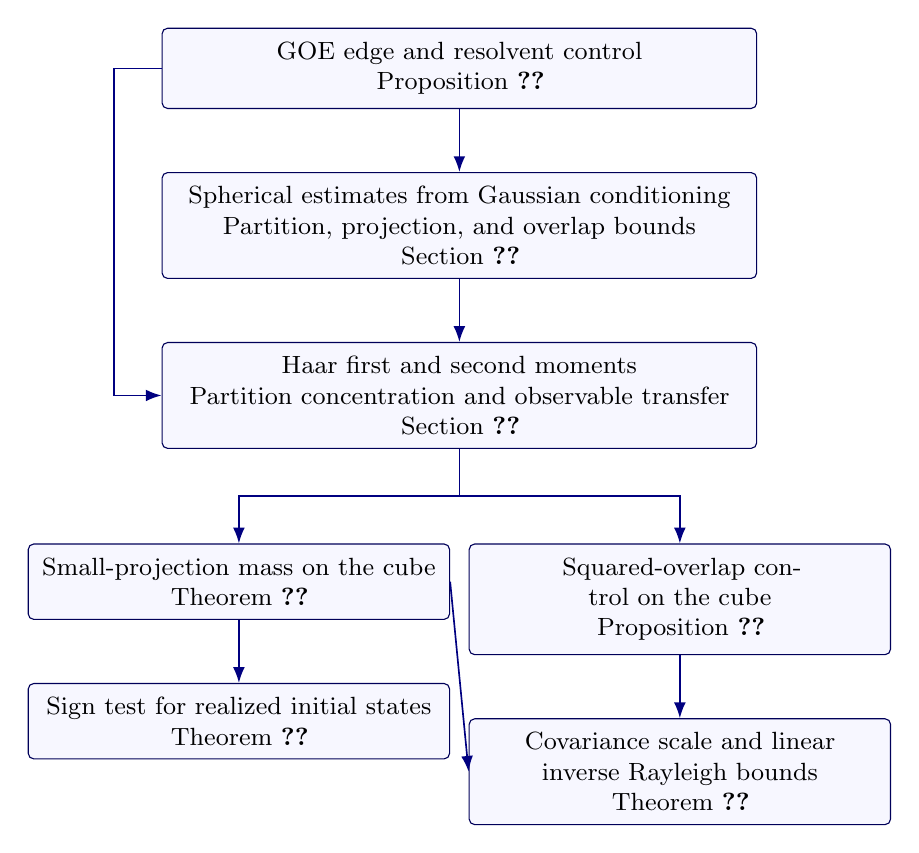
\begin{tikzpicture}[
 box/.style={draw=blue!35!black,rounded corners=2pt,fill=blue!3,
  text width=7.2cm,align=center,inner sep=5pt,font=\small},
 branch/.style={box,text width=5cm},
 flow/.style={-{Latex[length=2mm]},semithick,draw=blue!50!black}]
\node[box] (spec) {GOE edge and resolvent control\\Proposition~\ref{prop:spectral}};
\node[box,below=8mm of spec] (sphere) {Spherical estimates from Gaussian conditioning\\Partition, projection, and overlap bounds\\Section~\ref{sec:spherical}};
\node[box,below=8mm of sphere] (cube) {Haar first and second moments\\Partition concentration and observable transfer\\Section~\ref{sec:orientation}};
\node[branch,anchor=north] (small) at ([xshift=-2.8cm,yshift=-12mm]cube.south) {Small-projection mass on the cube\\Theorem~\ref{thm:static-small-ball}};
\node[branch,anchor=north] (cov) at ([xshift=2.8cm,yshift=-12mm]cube.south) {Squared-overlap control on the cube\\Proposition~\ref{prop:overlap}};
\node[branch,below=8mm of small] (slow) {Sign test for realized initial states\\Theorem~\ref{thm:gibbs-start}};
\node[branch,below=8mm of cov] (lin) {Covariance scale and linear\\inverse Rayleigh bounds\\Theorem~\ref{thm:linear-scale}};
\draw[flow] (spec)--(sphere);
\draw[flow] (sphere)--(cube);
\draw[flow] (spec.west)--++(-6mm,0)|-(cube.west);
\draw[flow] (cube.south)--++(0,-.6)-|(small.north);
\draw[flow] (cube.south)--++(0,-.6)-|(cov.north);
\draw[flow] (small)--(slow);
\draw[flow] (cov)--(lin);
\draw[flow] (small.east)--(lin.west);
\end{tikzpicture}
\caption{The lower and static argument. The direct arrow from the spectral estimates to Haar comparison records their additional use in the cubic overlap deficit. The restricted first moment transfers the small-projection numerator, while partition concentration controls its normalization; a weighted second moment transfers squared overlap. Small projections give the covariance lower bound and squared overlap gives its upper bound. A separate cavity estimate then controls the linear inverse Rayleigh quotients. The independent subexponential upper comparison is outside the diagram.}
\label{fig:proof-structure}
\end{figure}


\section{Model, clocks, and conventions}\label{sec:model}
This section fixes the normalization shared by the static and dynamical
arguments. In particular, adding a GOE diagonal will provide spectral
test vectors without changing any quantity intrinsic to the spin law.

Throughout, $n\to\infty$; arguments using three distinguished coordinates
are applied for $n\ge3$. Constants $c,C>0$ are independent of $n$, may
change from line to line, and have only the additional dependencies
explicitly indicated. Vector norms are Euclidean and matrix norms are
operator norms. We write $O_{\Prob}(1)$ for a sequence whose laws are
tight. Equivalently, its absolute value exceeds any positive deterministic
divergent threshold with probability tending to zero. The ability to
test every such threshold will be used in the covariance argument.

Following the Gaussian diagonal augmentation in
\cite[Equation~(1.1)]{comets1996}, let $W$ be a real symmetric GOE matrix
with independent entries on and above its diagonal, with
\[
 W_{ij}\sim N(0,1/n)\quad(i<j),\qquad
 W_{ii}\sim N(0,2/n).
\]
Set $\Omega_n=\{-1,1\}^n$ and
\[
 H_W(x)=\tfrac12x^TWx,
 \qquad
 \mu_W(x)=\frac{e^{H_W(x)}}{\sum_{y\in\Omega_n}e^{H_W(y)}}.
\]
We abbreviate $\mu_W$ to $\mu$ when the disorder is fixed. Because every $x_i^2=1$, the diagonal contributes the same quantity
$\frac12\sum_iW_{ii}$ to every configuration. It cancels from the Gibbs
normalization, leaving precisely \eqref{eq:intro-law}. Covariance,
heat-bath kernels and mixing times therefore depend only on the original
off-diagonal disorder. A spectral direction may still depend on the added
diagonal. In the realized-start proof we use that direction to test an
intrinsic total-variation distance, and only then integrate out the
diagonal. This distinction avoids imposing an unnecessary simultaneous
choice of a test direction for all initial states.

For functions $f,g:\Omega_n\to\R$, write
\[
 \langle f,g\rangle_\mu=\mu[fg],
 \qquad
 P_i f=\E_\mu[f\mid x_{-i}],
 \qquad
 \mathcal L=\sum_{i=1}^n(P_i-\mathrm{Id}),
 \quad P=\frac1n\sum_{i=1}^nP_i.
\]
The two transition operators are $e^{t\mathcal L}$ and $P^k$.
Their exact relation is $\mathcal L=n(P-\mathrm{Id})$; time in one clock
must therefore not be read as a number of attempts in the other.
Every conditional spin probability is positive. Single-site updates
connect the cube, and the discrete chain can hold, so both chains are
irreducible and the discrete chain is aperiodic.

\begin{lemma}[Heat-bath forms]\label{lem:heatbath-form}
Each $P_i$ is an orthogonal projection in $L^2(\mu)$. The unscaled Dirichlet form is
\begin{align}
 \mathcal D_\mu(f)
 &=-\langle f,\mathcal Lf\rangle_\mu
   =\sum_i\mu[(f-P_if)^2]  \label{eq:heatbath-form}\\
 &=\sum_i\inf_{h_i:\{-1,1\}^{n-1}\to\R}
       \mu[(f-h_i(x_{-i}))^2].\nonumber
\end{align}
The discrete form is $\langle f,(\mathrm{Id}-P)f\rangle_\mu=\mathcal D_\mu(f)/n$, and $P$ has spectrum in $[0,1]$. For a linear function,
\begin{equation}\label{eq:linear-form}
 \mathcal D_\mu(a^Tx)=\sum_i a_i^2\alpha_i,
 \qquad
 \alpha_i=\mu[\sech^2 g_i],\quad
 g_i(x)=\sum_{j\ne i}W_{ij}x_j.
\end{equation}
\end{lemma}
\begin{proof}
Conditional expectation is the orthogonal projection onto functions of
$x_{-i}$. Hence
$\langle f,(\mathrm{Id}-P_i)f\rangle_\mu=\|f-P_if\|_{L^2(\mu)}^2$,
and this squared distance is the infimum over all such functions.
Summing proves \eqref{eq:heatbath-form}; averaging instead proves the
discrete form identity. Moreover
$0\le\langle f,Pf\rangle_\mu\le\langle f,f\rangle_\mu$ for every $f$,
so the spectrum of $P$ lies in $[0,1]$.

For a linear observable, all terms except $a_ix_i$ are fixed after
conditioning on $x_{-i}$. The conditional mean and variance of $x_i$
are $\tanh g_i$ and $\sech^2g_i$, respectively. Its contribution to the
form is therefore $a_i^2\mu[\sech^2g_i]$, which gives
\eqref{eq:linear-form}.
\end{proof}

For probability laws $\nu,\mu$ on $\Omega_n$, use
\[
 \|\nu-\mu\|_{\TV}
 =\tfrac12\sum_x|\nu(x)-\mu(x)|
 =\sup_{A\subseteq\Omega_n}|\nu(A)-\mu(A)|.
\]
Define
\begin{align*}
 d_t^{\rm ct}(W,x)&=\|e^{t\mathcal L}(x,\cdot)-\mu_W\|_{\TV},&
 t_{\rm mix}&=\inf\{t\ge0:\max_xd_t^{\rm ct}(W,x)\le1/4\},\\
 d_k^{\rm dt}(W,x)&=\|P^k(x,\cdot)-\mu_W\|_{\TV},&
 k_{\rm mix}&=\min\{k\in\N\cup\{0\}:\max_xd_k^{\rm dt}(W,x)\le1/4\}.
\end{align*}
All limits in probability and statements holding with high probability refer to the disorder, together with explicitly introduced auxiliary randomness. No uniform assertion over disorder-adaptive time sequences is implicit.

We finish with the static identity that will turn overlap bounds into
covariance bounds. Zero field gives $\mu(x)=\mu(-x)$, so every spin has
mean zero. Consequently
\[
 \Sigma=\Cov_\mu(x)=\mu[xx^T],\qquad
 \Sigma_{ii}=1,
 \qquad q(x,y)=\frac{x^Ty}{n}.
\]
For independent samples from $\mu$, expansion of the square gives
\begin{equation}\label{eq:overlap-covariance}
 \Tr\Sigma^2=n^2\E_{\mu\otimes\mu}q^2.
\end{equation}

\section{Spectral estimates at a slowly enlarged edge scale}
\label{sec:spectral}

Our objective is to control the leading GOE eigenvalues and the first
two resolvent traces just above the edge on an event independent of
eigenvector orientation. These estimates enter both the Gaussian
conditioning argument in Section~\ref{sec:spherical} and the variational
deficit in Section~\ref{sec:orientation}. A fixed logarithmic enlargement
would lose the strongest quantifiers of the main theorems, so the
enlargement below may diverge as slowly as needed.

The proof has three parts. Tridiagonalization isolates independent noise;
a simultaneous quadratic-form estimate compares that noise with a
deterministic confinement energy; and a Hermite identity evaluates the
deterministic resolvent. Here $C,c>0$ are universal, while $C_M$ may also
depend on a fixed $M<\infty$.

Let $L_n\to\infty$ be any positive deterministic sequence with $L_n\le\log n$ for
all sufficiently large $n$, and set
\begin{equation}
 s_*=n^{-2/3},\qquad s_0=L_ns_*,\qquad
 h_n=L_n^{1/8},\qquad
 A_n=h_n+\sqrt{\log(2+L_n)},\qquad
 \eta_n=A_nL_n^{-3/4}.
 \label{eq:spectral-scales}
\end{equation}
In particular, $\eta_n\to0$.  Define
\[
 R(s)=\frac{2+s-\sqrt{s(4+s)}}2,\qquad s>0.
\]

\begin{proposition}[An eigenvalue-only good event]
\label{prop:spectral}
Let $W$ have the GOE normalization of Section~\ref{sec:model}, and write its
eigenvalues as $\lambda_1\ge\cdots\ge\lambda_n$.  There are events
$\mathcal G_n(L_n)$, measurable with respect to these eigenvalues alone,
such that
\[
 \Prob\bigl(\mathcal G_n(L_n)^c\bigr)
 \le C\exp(-cL_n^{1/4})
\]
for all sufficiently large $n$.  On the same events, for every fixed
$M<\infty$,
\begin{equation}
\begin{aligned}
 &\lambda_j=2+o(s_0)\quad(1\le j\le3),
 &&\max_i|\lambda_i|\le3,\\
 &\frac1n\sum_{i=1}^n\frac1{2+s-\lambda_i}
     =R(s)+o(\sqrt s),
 &&\frac1n\sum_{i=1}^n\frac1{(2+s-\lambda_i)^2}
     \le\frac{C_M}{\sqrt s}
 \quad(s_0\le s\le M).
\end{aligned}
\label{eq:spectral-estimates}
\end{equation}
All denominators in these formulas are positive.  The little-oh terms have
deterministic bounds, uniformly over the event: the first three eigenvalue
errors divided by $s_0$ are at most $C(L_n^{-1}+\eta_n)$, and the first
resolvent error divided by $\sqrt s$ is at most
$C_M(L_n^{-3/2}+\eta_n)$.  The event does not depend on $M$.
\end{proposition}

\subsection{Tridiagonal reduction and concentration of its entries}

The following reduction is the GOE tridiagonalization of
\cite[Theorem~2.1]{dumitriuEdelman2002}. We include the argument to fix both its
normalization and its independence properties.

\begin{lemma}[Tridiagonal representation]
\label{lem:tridiagonal}
The eigenvalues of $W$ have the same law as those of a symmetric
tridiagonal matrix $T$ whose entries
\[
 T_{ii}\sim N(0,2/n),\qquad
 T_{i,i+1}=T_{i+1,i}\sim\frac{\chi_{n-i}}{\sqrt n}
 \quad(1\le i<n)
\]
are independent.  Here $\chi_m$ is the Euclidean norm of $m$ independent
standard normal variables.
\end{lemma}

\begin{proof}
We expose one column at a time. The first diagonal entry, the rest of
the first column, and the trailing square block are independent; this
independence will persist after each rotation.  The column vector has $n-1$ independent $N(0,1/n)$ entries.
Choose an orthogonal transformation of the trailing coordinates that sends
this vector to its nonnegative length times the first coordinate vector.
Conjugation by this transformation produces the desired first
off-diagonal entry.

To justify the next exposure, observe that the trailing block has
density proportional to $\exp(-n\Tr B^2/4)$. Both this density and
Euclidean volume are invariant under orthogonal conjugation.  Conditional on the
column vector, the chosen transformation is fixed, so the conjugated
trailing block still has the same GOE density and its conditional law does
not depend on the column.  It is therefore independent of all entries
already exposed.  Repeat the construction inside that block, then inside
each successive trailing block.  At step $i$ the fresh column has $n-i$
independent $N(0,1/n)$ entries.  This proves both the stated distributions
and their joint independence.  The conjugations preserve eigenvalues.
\end{proof}

The reduction leaves Gaussian diagonal noise and centered chi noise
off the diagonal. Both satisfy a dimension-independent exponential
estimate. For the latter, the two estimates we need are
\begin{equation}
 \E\exp\left(t\frac{\chi_m-\E\chi_m}{\sqrt n}\right)
 \le \exp(Ct^2/n),\qquad
 0\le\sqrt m-\E\chi_m\le\frac C{\sqrt m}.
 \label{eq:chi-entry-bounds}
\end{equation}
Here and below a moment-generating bound is asserted for every real $t$.
For completeness, the Gaussian-square moment-generating function and
Chernoff's inequality give
\[
 \Prob\{\chi_m^2\ge ma\}\le(ae^{1-a})^{m/2}
 \quad(a>1),
\]
with the same right-hand side for the lower-tail event when $0<a<1$.
Since
\[
 a-1-\log a\ge(\sqrt a-1)^2,
\]
it follows that
$\Prob\{|\chi_m-\sqrt m|\ge r\}\le2e^{-r^2/2}$ for $r\ge0$.
This tail bound gives $\Var(\chi_m)\le C$ and, by Jensen's inequality,
\[
 \sqrt m-\E\chi_m
 =\frac{\Var(\chi_m)}{\sqrt m+\E\chi_m}\le\frac C{\sqrt m}.
\]
To prove the centered exponential bound without an extra prefactor, let
$X,X'$ be independent copies of $\chi_m$ and put $Z=X-X'$.  Then $Z$ is
symmetric and
\[
 \Prob\{|Z|\ge r\}\le4e^{-r^2/8},\qquad
 \E Z^{2k}\le4\cdot8^k k!\quad(k\ge1).
\]
The moment bound follows by integrating the tail.  Jensen's inequality
conditional on $X$, followed by the power series of $\cosh$, gives
\[
\begin{aligned}
 \E e^{t(X-\E X)}
 &\le\E e^{tZ}=\E\cosh(tZ)\\
 &\le1+4\sum_{k\ge1}\frac{8^k k!t^{2k}}{(2k)!}
 \le1+4(e^{8t^2}-1)\le e^{32t^2}.
\end{aligned}
\]
We used $(2k)!\ge(k!)^2$ and $(1+u)^4\ge1+4u$ for $u\ge0$.
The Gaussian tail ensures exponential integrability, and Tonelli's theorem
also justifies the nonnegative $\cosh$ series.  Replacing $t$ by
$t/\sqrt n$ proves~\eqref{eq:chi-entry-bounds}.  The centered diagonal
entries satisfy the same exponential estimate directly.

\subsection{A simultaneous quadratic-form estimate}

The quadratic-form estimate follows the approach used in soft-edge analysis for
tridiagonal ensembles. Ram\'irez, Rider, and Vir\'ag
\cite{ramirezRiderVirag2011} developed a variational approach involving
discrete gradient and confinement energies. The block summation-by-parts
estimate of Ledoux and Rider \cite[Proposition~7 and Lemma~8]{ledouxRider2010}
is particularly close to the noise control used here. Their proof of
Theorem~1 (Right-Tail), on page~1329 immediately before Lemma~9, gives
the corresponding substitution for off-diagonal weights. We arrange that control simultaneously
over energy scales and spatial shells, then use a deterministic Hermite
resolvent identity. This provides the first and second resolvent bounds
needed here for every slowly diverging edge enlargement.

Let $D$ be the deterministic tridiagonal matrix with zero diagonal and
off-diagonal entries
\[
 c_i=\sqrt{1-i/n}\quad(1\le i<n),\qquad E=2I-D.
\]
For later boundary formulas set $c_0=c_n=0$.

\begin{lemma}[Noise controlled by deterministic energy]
\label{lem:form-bound}
There is a universal constant $C_0$ such that, with
\[
 \Phi_n(x)=C_0n^{-1/2}A_n(x+s_0)^{1/4}
             \sqrt{1+\log(1+x/s_0)},\qquad x\ge0,
\]
the matrix $H=T-D$ satisfies, simultaneously for every unit vector
$u\in\R^n$,
\begin{equation}
 |u^THu|\le\Phi_n(u^TEu)
 \label{eq:form-bound}
\end{equation}
on an event $\mathcal F_n$ with
$\Prob(\mathcal F_n^c)\le C\exp(-cL_n^{1/4})$ for all sufficiently large $n$.
Moreover,
\begin{equation}
 \sup_{x\ge0}|\Phi_n'(x)|\le C\eta_n,
 \qquad \Phi_n(0)\le C\eta_ns_0.
 \label{eq:phi-smallness}
\end{equation}
\end{lemma}

\begin{proof}
We prove the lemma in three steps: the deterministic energy controls
where a vector can concentrate, one noise event controls block prefixes
at every relevant scale, and summation by parts combines these controls.

\smallskip\noindent\emph{Energy controls spatial mass and gradients.}
For a unit vector $u$, write $e=u^TEu$. Expanding gives
\begin{equation}
 e=\sum_{i<n}c_i(u_i-u_{i+1})^2
   +\sum_{i=1}^n(2-c_i-c_{i-1})u_i^2.
 \label{eq:deterministic-energy}
\end{equation}
The row sums of $D$ are at most two, so $0\le E\le4I$.  The coefficients
$2-c_i-c_{i-1}$ are at least $i/(2n)$: for interior indices this follows
from $1-\sqrt{1-t}\ge t/2$, and the boundary indices satisfy the same
inequality directly.  Also $c_i\ge1/\sqrt2$ when $i\le n/2$.
Thus~\eqref{eq:deterministic-energy} implies
\begin{equation}
 \sum_i\frac{i}{n}u_i^2\le2e,\qquad
 \sum_{i>n/2}u_i^2+
 \sum_{i<n}(u_i-u_{i+1})^2\le Ce.
 \label{eq:energy-tail-gradient}
\end{equation}
For the second inequality, control gradients in the first half by the
weighted gradient term, and use
$(u_i-u_{i+1})^2\le2u_i^2+2u_{i+1}^2$ for the remaining edges.

\smallskip\noindent\emph{One event for every energy.}
The vector will be selected after the matrix has been realized, so the
probability estimate must be simultaneous. We first prepare blocks at
every dyadic energy scale. Set
\[
 \sigma_j=2^js_*,\qquad
 0\le j\le J_n:=\left\lceil\log_2(4/s_*)\right\rceil,
 \qquad d_j=\max\{1,\lfloor\sigma_j^{-1/2}\rfloor\}.
\]
For each of the two independent-entry sequences (diagonal entries and
centered off-diagonal entries), partition its index set into consecutive
blocks of lengths between $d_j$ and $2d_j$.  Such a partition is obtained
by merging a last short block with its predecessor.  Assign label $r=0$
when the first index of a block is at most $2n\sigma_j$; otherwise assign
$r\ge1$ when that index is in
$(2^rn\sigma_j,2^{r+1}n\sigma_j]$.

If $\xi_i$ is either centered entry sequence and a block has length
$m\le2d_j$, its partial sums $S_k$ obey
\[
 \Prob\left\{\max_{k\le m}|S_k|\ge a\right\}
 \le2\exp\left(-\frac{na^2}{C d_j}\right).
\]
Indeed, $\exp(tS_k-Ckt^2/n)$ is a nonnegative supermartingale by
\eqref{eq:chi-entry-bounds}.  Stopping it at its first crossing of $a$
bounds the one-sided probability by
$\exp(-ta+Cmt^2/n)$; optimizing $t>0$ and repeating for $-S_k$ proves
the displayed estimate.

At a fixed pair $(j,r)$, the number of blocks is at most
\[
 C\left(1+\frac{2^rn\sigma_j}{d_j}\right)
 \le C2^rn\sigma_j^{3/2}=C2^{r+3j/2}.
\]
For $\sigma_j\le1$, use $d_j\ge\sigma_j^{-1/2}/2$; for
$\sigma_j>1$, use $d_j=1$.  The additive constant is absorbed because
$n\sigma_j^{3/2}\ge1$.  Consequently, for a sufficiently large fixed
constant $K$, there is an event $\mathcal F_n$ on which every block of
both sequences has all its centered partial sums bounded by
\begin{equation}
 K\sqrt{d_j/n}\,(h_n+\sqrt{j+r}),
 \label{eq:block-prefix}
\end{equation}
and
\[
\begin{aligned}
 \Prob(\mathcal F_n^c)
 &\le C\sum_{j,r\ge0}2^{r+3j/2}
       e^{-cK^2(h_n+\sqrt{j+r})^2}\\
 &\le C e^{-c'h_n^2}=C e^{-c'L_n^{1/4}}.
\end{aligned}
\]
Here $K$ is chosen so that the factors in $j$ and $r$ form summable
geometric series.  This bound does not acquire a factor from the number
of scales.

\smallskip\noindent\emph{From block prefixes to quadratic forms.}
We may now fix the noise event and choose an arbitrary unit vector.
Select the first $j$ for which $e\le\sigma_j$. Since $e\le4$, this
index exists, and
\[
 \sigma_j\le2(e+s_*).
\]
For the weights $w_i=u_i^2$ or $w_i=u_iu_{i+1}$, the sum of their
absolute values over all blocks with label $r$ is at most $C2^{-r}$.
For $r\ge1$, every coordinate used is beyond $2^rn\sigma_j$, and
\eqref{eq:energy-tail-gradient} bounds its total squared mass by
$2e/(2^r\sigma_j)\le2^{1-r}$.  The off-diagonal weights obey the same
bound by $|u_iu_{i+1}|\le(u_i^2+u_{i+1}^2)/2$.  For $r=0$, use the
unit norm.

The summed variation of these weights within those blocks is at most
$C2^{-r/2}\sqrt e$.  To verify this assertion, use
\[
 u_{i+1}^2-u_i^2=(u_{i+1}-u_i)(u_{i+1}+u_i)
\]
for diagonal weights and
\[
 u_{i+1}u_{i+2}-u_iu_{i+1}
 =u_{i+1}\bigl[(u_{i+2}-u_{i+1})+(u_{i+1}-u_i)\bigr]
\]
for off-diagonal weights.  Cauchy--Schwarz combines the preceding tail
mass bound with the total gradient bound in
\eqref{eq:energy-tail-gradient}; each coordinate or edge is counted at
most a fixed number of times.

For clarity, the summation-by-parts step can be made blockwise.  Suppose
all centered entry prefixes in a block are bounded by $B$, and let
$\bar\xi$ be the entry average on that block.  Then
$|\bar\xi|\le B/d_j$.  The prefixes of $\xi_i-\bar\xi$ are at most
$2B$ and vanish at the block end.  Therefore
\[
 \left|\sum_{i\text{ in block}}\xi_iw_i\right|
 \le\frac B{d_j}\sum_{i\text{ in block}}|w_i|
      +2B\sum_{\substack{i,i+1\text{ in block}}}|w_{i+1}-w_i|.
\]
Using~\eqref{eq:block-prefix} and summing by labels proves that either
centered weighted sum is bounded by
\begin{align*}
 &C n^{-1/2}\sum_{r\ge0}(h_n+\sqrt{j+r})
 \left(d_j^{-1/2}2^{-r}+d_j^{1/2}2^{-r/2}\sqrt e\right)\\
 &\hspace{35mm}\le C(h_n+\sqrt j)n^{-1/2}\sigma_j^{1/4}.
\end{align*}
For $\sigma_j\le1$, the last step uses
$d_j\asymp\sigma_j^{-1/2}$ and $e\le\sigma_j$.  For
$1<\sigma_j<8$, it follows from $d_j=1$ with a changed universal
constant.  The series in $r$ converges geometrically, including its
$\sqrt r$ factor.

The centered entries have now been controlled uniformly in $u$.
The only remaining part of $T-D$ is the deterministic error in the
off-diagonal means. By
\eqref{eq:chi-entry-bounds}, their difference from $c_i$ is at most
$C/(\sqrt n\sqrt{n-i})$.  It is at most $C/n$ for $i\le n/2$ and at
most $C/\sqrt n$ thereafter.  Thus their quadratic-form contribution is
at most
\[
 C/n+Ce/\sqrt n,
\]
using again the tail mass bound.  Finally,
\[
 j\le C\log(2+e/s_*)
 \le C\bigl[\log(2+L_n)+\log(1+e/s_0)\bigr].
\]
Together with $\sigma_j\le2(e+s_*)$ and $s_*\le s_0$, this converts
the centered estimate into~\eqref{eq:form-bound}.  The mean errors are
absorbed into the same bound because $0\le e\le4$ and $L_n\ge1$ for
large $n$.  Both sequences, and the factor two from off-diagonal entries,
are absorbed by choosing $C_0$ once and for all.

Finally, the scalar comparison must be stable under changing the
energy. Put $q(x)=1+\log(1+x/s_0)$. Direct differentiation gives
\[
 \Phi_n'(x)=C_0n^{-1/2}A_n(x+s_0)^{-3/4}
 \left(\frac{\sqrt{q(x)}}4+\frac1{2\sqrt{q(x)}}\right).
\]
Since $y^{-3/4}\sqrt{1+\log y}$ is bounded for $y\ge1$, its supremum
is at most $Cn^{-1/2}A_ns_0^{-3/4}=C\eta_n$.
The equality $\Phi_n(0)/s_0=C_0\eta_n$ proves the other assertion in
\eqref{eq:phi-smallness}.
\end{proof}

\subsection{The deterministic resolvent}
The noise bound reduces the random trace problem to $D$. Its entries
were chosen so that the characteristic polynomials satisfy a Hermite
recurrence. The resulting scalar differential equation will control both
the resolvent and the number of eigenvalues near the edge.

\begin{lemma}[Hermite resolvent estimates]
\label{lem:deterministic-resolvent}
Let $e_1\le\cdots\le e_n$ be the eigenvalues of $E=2I-D$, and set
\[
 R_D(s)=\frac1n\Tr(s+E)^{-1},\qquad
 T_D(s)=\frac1n\Tr(s+E)^{-2}=-R_D'(s).
\]
For every fixed $M<\infty$ and all sufficiently large $n$, uniformly for
$s_0\le s\le M$,
\begin{equation}
 T_D(s)\le C_Ms^{-1/2},\qquad
 0\le R(s)-R_D(s)\le\frac{C_M}{ns}.
 \label{eq:deterministic-traces}
\end{equation}
Moreover,
\begin{equation}
 N(t):=\#\{i:e_i\le t\}\le Cnt^{3/2}
 \qquad(t\ge s_0).
 \label{eq:deterministic-counting}
\end{equation}
\end{lemma}

\begin{proof}
We first derive the differential equation and locate its relevant
quadratic root, then absorb its finite-dimensional error at $s\ge s_0$.
Reverse the coordinates of $D$. Its off-diagonal entries become
$\sqrt{k/n}$, $1\le k<n$, so the characteristic polynomials of its
successive principal minors satisfy
\[
 P_0(z)=1,\quad P_1(z)=z,\quad
 P_{k+1}(z)=zP_k(z)-(k/n)P_{k-1}(z).
\]
Induction gives $P_k'=kP_{k-1}$: differentiation of the recurrence and
the recurrence one step earlier show that
$P_{k+1}'=P_k+kP_k$.  Consequently
\[
 P_n''-nzP_n'+n^2P_n=0.
\]
Since $P_n$ is the characteristic polynomial of $D$,
$R_D(s)=P_n'(2+s)/(nP_n(2+s))$.  The differential equation yields
\begin{equation}
 R_D(s)^2-(2+s)R_D(s)+1=\frac{T_D(s)}n>0.
 \label{eq:hermite-riccati}
\end{equation}
For every $s>0$, $R_D(s)$ is finite because $E\ge0$.
The two roots of the quadratic on the left are $R(s)$ and
\[
 R_+(s)=\frac{2+s+\sqrt{s(4+s)}}2.
\]
At large $s$, $R_D(s)\to0$ whereas $R_+(s)\to\infty$.  Positivity
in~\eqref{eq:hermite-riccati} thus places $R_D$ below the smaller root
there, and continuity prevents it from crossing either root anywhere on
$(0,\infty)$.  If $\delta(s)=R(s)-R_D(s)$, factoring the quadratic gives
\begin{equation}
 0\le\delta(s)\le
 \frac{T_D(s)}{n\sqrt{s(4+s)}}.
 \label{eq:root-difference}
\end{equation}

Termwise comparison of resolvents shows that
\[
 T_D(s)\le\frac2s\bigl[R_D(s/2)-R_D(s)\bigr]
 \le\frac2s\bigl[R(s/2)-R(s)+\delta(s)\bigr].
\]
Differentiating the explicit expression for $R$ gives
\[
 0<-R'(s)=\frac{2}{\sqrt{s(4+s)}\,
          (2+s+\sqrt{s(4+s)})}\le\frac1{2\sqrt s}.
\]
Integrating from $s/2$ to $s$ therefore gives
$R(s/2)-R(s)\le\sqrt s-\sqrt{s/2}\le\sqrt s$.  Hence
\[
 T_D(s)\le\frac C{\sqrt s}
       +\frac{2T_D(s)}{ns\sqrt{s(4+s)}}.
\]
For $s\ge s_0$, the coefficient of the last term is at most
$(ns_0^{3/2})^{-1}=L_n^{-3/2}\to0$.  Absorbing it proves the bound on
$T_D$, and~\eqref{eq:root-difference} then proves the bound on
$\delta$.  Notice that $R_D(s/2)\le R(s/2)$ was established for every
positive $s/2$; it does not require $s/2\ge s_0$.

The second-trace estimate also gives the counting estimate needed for
the later dyadic transfer. For $s_0\le t\le1$, each $e_i\le t$
contributes at least
$(2t)^{-2}$ to $nT_D(t)$.  Thus
$N(t)\le4nt^2T_D(t)\le Cnt^{3/2}$.  For $t\ge1$, the same bound
follows from $N(t)\le n$.
\end{proof}

\subsection{Eigenvalue comparison and transfer of the traces}

\begin{proof}[Proof of Proposition~\ref{prop:spectral}]
The previous lemmas supply the noise control and the reference traces.
We now transfer them to an event defined entirely by the eigenvalues.
There are three tasks: compare ordered eigenvalues, locate the top three,
and compare the two traces.

\smallskip\noindent\emph{Ordered eigenvalues.}
Work first in the tridiagonal realization. On $\mathcal F_n$,
\eqref{eq:form-bound} bounds the Rayleigh quotient of $E-H=2I-T$ between
\[
 f_-(e):=e-\Phi_n(e)\quad\hbox{and}\quad f_+(e):=e+\Phi_n(e).
\]
By~\eqref{eq:phi-smallness}, both functions are increasing for large $n$.
The span of the first $i$ eigenvectors of $E$ has every unit-vector
energy at most $e_i$, so the min--max principle gives
$2-\lambda_i\le f_+(e_i)$.  On the span of eigenvectors $i$ through
$n$, every energy is at least $e_i$; the complementary max--min
principle gives $2-\lambda_i\ge f_-(e_i)$.  Therefore
\begin{equation}
 |2-\lambda_i-e_i|\le\Phi_n(e_i),\qquad 1\le i\le n.
 \label{eq:eigenvalue-comparison}
\end{equation}
This argument uses monotonicity of scalar functions of Rayleigh
quotients, and does not require an operator-monotonicity assertion.

Define $\mathcal G_n(L_n)$ to be precisely the event
\eqref{eq:eigenvalue-comparison}, with the deterministic $e_i$ and
$\Phi_n$ constructed above.  It depends only on the ordered eigenvalues.
The tridiagonal event $\mathcal F_n$ implies it; hence
Lemma~\ref{lem:tridiagonal} transfers its probability bound to $W$.
All remaining conclusions are deterministic on $\mathcal G_n(L_n)$.

\smallskip\noindent\emph{The first three directions.}
The conditioning argument will need three large coordinate variances.
To locate the corresponding eigenvalues, take
$m=\lfloor n^{1/3}\rfloor$ and the span of the first three discrete
Dirichlet sine modes on $\{1,\ldots,m\}$, extended by zero.
The Dirichlet Laplacian on this segment has eigenvalues
$4\sin^2(k\pi/[2(m+1)])$, so its quadratic form on this span is at most
$C/m^2$.  On vectors supported on the segment, the form difference
between $E$ and that Laplacian has absolute value at most
\[
 2\max_{1\le i<m}|1-c_i|\sum_{i<m}|u_iu_{i+1}|
 \le Cm/n.
\]
The min--max principle therefore gives
$0\le e_1,e_2,e_3\le C(m^{-2}+m/n)\le Cn^{-2/3}$.
Equations~\eqref{eq:phi-smallness} and
\eqref{eq:eigenvalue-comparison} imply
\[
 \max_{j\le3}\frac{|\lambda_j-2|}{s_0}
 \le C(L_n^{-1}+\eta_n).
\]
Also every $e_i\in[0,4]$, so
$\max_i|\lambda_i|\le2+\Phi_n(4)$.  The assumption $L_n\le\log n$
gives $\Phi_n(4)=o(1)$, proving the stated bound by three.

\smallskip\noindent\emph{Resolvent traces.}
The eigenvalue comparison also controls every denominator: for every
$s\ge s_0$ and every $e\in[0,4]$,
\begin{equation}
 \frac{\Phi_n(e)}{s+e}
 \le\frac{\Phi_n(0)+C\eta_ne}{s+e}
 \le C\eta_n.
 \label{eq:denominator-comparison}
\end{equation}
Thus~\eqref{eq:eigenvalue-comparison} makes
$2+s-\lambda_i$ positive and equal to $(s+e_i)(1+O(\eta_n))$,
uniformly in both $i$ and $s\ge s_0$.
The normalized second trace is consequently at most a constant times
$T_D(s)$, proving its bound in~\eqref{eq:spectral-estimates}.

For the first trace, subtract term by term and use
$(e_i+s_0)^{1/4}\le(s+e_i)^{1/4}$ to obtain
\begin{align}
 &\left|\frac1n\sum_i\frac1{2+s-\lambda_i}-R_D(s)\right|\notag\\
 &\qquad\le Cn^{-1/2}A_n\frac1n\sum_i
 (s+e_i)^{-7/4}\sqrt{1+\log(1+e_i/s_0)}.
 \label{eq:trace-perturbation}
\end{align}
We spell out the dyadic sum because its uniformity near $s_0$ is useful.
The range $e_i\le s$ contributes at most
\[
 Cs^{-7/4}\frac{N(s)}n\sqrt{1+\log(1+s/s_0)}
 \le Cs^{-1/4}\sqrt{1+\log(1+s/s_0)}.
\]
For $k\ge0$, the shell $2^ks<e_i\le2^{k+1}s$ contributes at most
\[
 Cs^{-1/4}2^{-k/4}
 \sqrt{1+\log(1+s/s_0)+(k+1)\log2},
\]
by~\eqref{eq:deterministic-counting}.  This counting estimate remains
valid above one, so all shells are covered.  The convergent geometric
series, with its additional square-root factor, bounds the sum in
\eqref{eq:trace-perturbation} by
\[
 C_Ms^{-1/4}\sqrt{1+\log(1+s/s_0)}.
\]
Dividing the resulting trace error by $\sqrt s$ and writing $r=s/s_0$
gives
\[
 C_M\eta_n r^{-3/4}\sqrt{1+\log(1+r)}\le C_M\eta_n
 \qquad(r\ge1).
\]
Finally, Lemma~\ref{lem:deterministic-resolvent} gives
\[
 \frac{|R_D(s)-R(s)|}{\sqrt s}
 \le\frac{C_M}{ns^{3/2}}\le C_ML_n^{-3/2}.
\]
This proves the quantitative first-trace error and completes all of
\eqref{eq:spectral-estimates}.  The event was defined before $M$ was
chosen, and each displayed error is deterministic on that event.
Consequently every deterministic sequence of spectra in
$\mathcal G_n(L_n)$ satisfies the estimates for every fixed finite $M$,
without any condition on eigenvector orientation.
\end{proof}

\section{Gaussian conditioning on the sphere}
\label{sec:spherical}

Conditioning independent centered Gaussian coordinates on their squared radius
gives an exact representation of a quadratic tilt of uniform sphere
measure. We quantify that representation in two stages. For bounded
deterministic spectra, radial-density estimates compare partition
integrals on the full sphere and its intersections with hyperplanes
through the origin with the same variational value. We then impose the
edge estimates of Section~\ref{sec:spectral} to bound small coordinate
projections and squared overlaps at criticality.

\subsection{Radial representation and partition estimates}

We begin with a deterministic ordered spectrum
$\lambda_1\ge\cdots\ge\lambda_n$, where $n\ge3$ and
$\max_i|\lambda_i|\le3$, and set
$\Lambda=\diag(\lambda_1,\ldots,\lambda_n)$.
Let $\sigma_n$ be uniform probability on
$\{u\in\R^n:\|u\|^2=n\}$.  For $0\le a\le2$, define
\begin{equation}
\label{eq:spherical-definitions}
 S(a)=\int e^{a u^T\Lambda u/2}\,\sigma_n(du),
 \qquad
 B(a)=\inf_{z>a\lambda_1}
 \left\{\frac{z-1}{2}
       -\frac1{2n}\sum_{i=1}^n\log(z-a\lambda_i)\right\}.
\end{equation}
The associated tilted probability is
\[
 \sigma_{\Lambda,a}(du)
 =S(a)^{-1}e^{a u^T\Lambda u/2}\,\sigma_n(du),
 \qquad
 \sigma_\Lambda=\sigma_{\Lambda,1}.
\]
Quadratic exponential laws on a sphere belong to the Bingham family
\cite{bingham1974}. Their representation through a Gaussian conditioned
on its radius, and the associated radial-density formula, are classical
in the analysis of Bingham and Fisher--Bingham normalizing constants
\cite{kumeWood2005,kumePrestonWood2013}. Gaussian integration and spherical
saddles also enter the SK analyses of Baik and Lee \cite{baikLee2016},
Landon \cite{landon2022}, and Du and Huang
\cite{duHuang2026FreeEnergy,duHuang2026Overlap}; the proof of Lemma~4.5 in
\cite{duHuang2026Overlap} uses the same representation by Gaussian
coordinates conditioned on the radius. We prove the exact identity
with the probability normalization and squared radius used here; no
saddlepoint approximation is used in this conditioning step.

\begin{lemma}[Gaussian representation]
\label{lem:spherical-identity}
For every $a\in[0,2]$, the infimum defining $B(a)$ has a unique minimizer
$z_a$.  With
\begin{equation}
\label{eq:spherical-saddle}
 k_i(a)=(z_a-a\lambda_i)^{-1},
 \qquad
 \sum_{i=1}^n k_i(a)=n,
\end{equation}
one has
\[
 1+a\lambda_n\le z_a\le1+a\lambda_1,
 \qquad
 \frac1{13}\le k_i(a)\le n.
\]
Let $Y_i$ be independent $N(0,k_i(a))$ variables, and let $p_a$ be the
density of $\sum_iY_i^2$.  Then
\begin{equation}
\label{eq:spherical-identity}
 S(a)=e^{nB(a)}
       \frac{p_a(n)}{p_{\chi_n^2}(n)}.
\end{equation}
The conditional law of $Y$ given $\|Y\|^2=n$, defined by radial
disintegration, is $\sigma_{\Lambda,a}$.
\end{lemma}

\begin{proof}
First choose the Gaussian variances so that the squared radius has
mean $n$. Then compare its radial density with the standard Gaussian
density at that same radius. To implement the first step, denote the
objective in \eqref{eq:spherical-definitions} by $F_a(z)$. On
$z>a\lambda_1$,
\[
 F_a'(z)=\frac12-\frac1{2n}\sum_i(z-a\lambda_i)^{-1},
 \qquad
 F_a''(z)=\frac1{2n}\sum_i(z-a\lambda_i)^{-2}>0.
\]
The derivative tends to $-\infty$ at the left endpoint and to $1/2$
at infinity.  The function itself tends to $+\infty$ at both ends.
This proves existence, uniqueness, and \eqref{eq:spherical-saddle}.

The average of the reciprocals of $z_a-a\lambda_i$ is one.  Their
minimum is therefore at most one, and their maximum is at least one,
giving the stated bounds on $z_a$.  Consequently
\[
 0<z_a-a\lambda_i
 \le1+a(\lambda_1-\lambda_n)\le13.
\]
The lower bound for $k_i(a)$ follows; the upper bound follows from
their positivity and sum $n$.  At $a=0$ these formulas give
$z_0=1$, $k_i(0)=1$, and $B(0)=0$.

The minimizer is now fixed. The radial comparison itself is exact
at any admissible $z$: put $Q=zI-a\Lambda$ and let
$Y^{z,a}\sim N(0,Q^{-1})$.  Its density relative to a standard
Gaussian vector at $y\in\R^n$ is
\[
 (\det Q)^{1/2}
 \exp\left(-\frac{z-1}{2}\|y\|^2+\frac a2y^T\Lambda y\right).
\]
The standard Gaussian has uniform conditional angular law.  Integrating
this ratio over the sphere of squared radius $n$ gives
\begin{equation}
\label{eq:spherical-radial-ratio}
 \frac{p_{z,a}(n)}{p_{\chi_n^2}(n)}
 =(\det Q)^{1/2}e^{-n(z-1)/2}S(a),
\end{equation}
where $p_{z,a}$ is the density of $\|Y^{z,a}\|^2$.
This identity is a polar-coordinate identity between continuous radial
densities at a positive radius.  At $z=z_a$, its rearrangement is
\eqref{eq:spherical-identity}.  The same density ratio, with the radius
fixed, proves the assertion about the conditional law.
\end{proof}

We will repeatedly use the two-square smoothing calculation also appearing in
\cite[Eq.~(7)]{BobkovNaumovUlyanov2021}.  If $G,H$ are
independent standard Gaussians and $d,e>0$, then the density
$r_{d,e}$ of $dG^2+eH^2$ satisfies
\begin{equation}
\label{eq:two-square-density}
 \begin{split}
 r_{d,e}(t)
 &=
 \frac1{2\pi\sqrt{de}}
 \int_0^t
 \frac{e^{-x/(2d)-(t-x)/(2e)}}{\sqrt{x(t-x)}}\,dx\\
 &\le \frac1{2\sqrt{de}},
 \qquad t>0.
 \end{split}
\end{equation}
The integral of $[x(t-x)]^{-1/2}$ over $(0,t)$ is $\pi$.
Convolving with further independent random variables preserves this
upper bound.

The next estimate is required at the mean of the weighted sum, including
arrays with a dominant weight. The Fourier majorant in its proof is the
weighted-square estimate of Bobkov, Naumov, and Ulyanov
\cite[Lemma~3]{BobkovNaumovUlyanov2021}, which we reproduce.
The compactness argument has the classical Gaussian-plus-quadratic
limiting structure described by Nourdin and Poly
\cite[Theorem~3.1]{NourdinPoly2012SecondChaos}; we give the needed
positive-weight argument directly. Their erratum
\cite{NourdinPoly2012Erratum} concerns separate finite-cumulant statements.

\begin{lemma}[Density at the mean]
\label{lem:mean-density}
There is a universal constant $c>0$ such that, for every $n\ge3$ and
every $k_1,\ldots,k_n>0$ with $\sum_i k_i=n$, the density $p$ of
$\sum_i k_iG_i^2$, for independent standard Gaussians $G_i$, satisfies
\begin{equation}
\label{eq:mean-density}
 p(n)\ge c\left(\sum_i k_i^2\right)^{-1/2}.
\end{equation}
\end{lemma}

\begin{proof}
After normalization, it is enough to exclude a sequence of densities
vanishing at zero. There are two ways such a sequence of weights can
behave: all weights vanish individually, giving a Gaussian limit, or a
positive largest weight remains and supplies a density bounded below
near zero. The proof treats these cases separately.

Set $\tau=(\sum_i k_i^2)^{1/2}$ and $d_i=k_i/\tau$. The centered
random variable
\[
 T_d=\sum_i d_i(G_i^2-1)
     =\frac{\sum_i k_iG_i^2-n}{\tau}
\]
has density $f_d$ with $f_d(0)=\tau p(n)$, and
$\sum_i d_i^2=1$.  Thus it suffices to bound $f_d(0)$ below uniformly
over all such finite arrays.  Each array has at least three positive
weights.  Its characteristic function is integrable, since its
absolute value decays as $O(|t|^{-n/2})$ at infinity; we always take
the resulting continuous version of its density.

Suppose, to the contrary, that arrays $d^{(r)}$ satisfy
$f_{d^{(r)}}(0)\to0$.  Sort each array in nonincreasing order and
extend it by zeros.  A diagonal subsequence has
$d_i^{(r)}\to c_i$ for every $i$, with
$\sum_i c_i^2\le1$.  We consider the two possible values of $c_1$.

\smallskip
\noindent\emph{Case $c_1=0$.}
For $d\ge0$, define
\[
 \psi_d(t)=\E e^{itd(G^2-1)}
          =e^{-itd}(1-2itd)^{-1/2}.
\]
For logarithms of characteristic functions, use the continuous
branch equal to zero at $t=0$.
For fixed $t$ and $|td|$ small, expansion gives
\[
 \log\psi_d(t)=-t^2d^2+O(|t|^3d^3).
\]
It follows that the characteristic function
$\phi_r(t)=\prod_i\psi_{d_i^{(r)}}(t)$ converges pointwise to
$e^{-t^2}$, because
$\sum_i(d_i^{(r)})^3\le d_1^{(r)}\sum_i(d_i^{(r)})^2=d_1^{(r)}$.

Weak convergence alone does not control a density at one point.
To pass through Fourier inversion we need an integrable bound uniform
in $r$. Concavity of $\log(1+x)$ and
$\sum_i(d_i^{(r)})^2=1$ give
\[
 |\phi_r(t)|
 =\prod_i\bigl(1+4(d_i^{(r)})^2t^2\bigr)^{-1/4}
 \le
 \bigl(1+4(d_1^{(r)})^2t^2\bigr)^{-1/(4(d_1^{(r)})^2)}.
\]
The function $x\mapsto \log(1+Ax)/x$ is decreasing for $A\ge0$.
Once $(d_1^{(r)})^2\le1/8$, the last expression is at most
$(1+t^2/2)^{-2}$.  Fourier inversion and dominated convergence imply
\[
 f_{d^{(r)}}(0)
 =\frac1{2\pi}\int_{\R}\phi_r(t)\,dt
 \longrightarrow
 \frac1{2\pi}\int_{\R}e^{-t^2}\,dt
 =\frac1{2\sqrt\pi},
\]
a contradiction.

\smallskip
\noindent\emph{Case $c_1>0$.}
Remove the largest coordinate and write
\[
 R_r=\sum_{i\ge2}d_i^{(r)}(G_i^2-1).
\]
We claim that $R_r$ converges in distribution to
\begin{equation}
\label{eq:density-residual-limit}
 R=\sum_{i\ge2}c_i(G_i^2-1)+Z,
 \qquad
 Z\sim N\left(0,\,2\left(1-\sum_{i\ge1}c_i^2\right)\right),
\end{equation}
where $Z$ and the displayed Gaussians are independent.
The series converges in $L^2$, since the tail beyond $m$ has variance
$2\sum_{i>m}c_i^2\to0$.  To identify the limit, note that the sorted weights
satisfy $d_{m+1}^{(r)}\le(m+1)^{-1/2}$.  For fixed $t$ and sufficiently
large $m$, the same logarithmic expansion as above gives, uniformly
in $r$,
\[
 \log\E e^{itR_r}
 =
 \sum_{i=2}^m\log\psi_{d_i^{(r)}}(t)
 -t^2\left(1-\sum_{i=1}^m(d_i^{(r)})^2\right)
 +O\left(\frac{|t|^3}{\sqrt{m+1}}\right).
\]
First let $r\to\infty$ and then $m\to\infty$.  The resulting
characteristic function is exactly that of \eqref{eq:density-residual-limit},
which proves the claim.

The residual limit has positive mass arbitrarily close to zero.
This is the fact that allows the surviving largest coordinate to
control the convolution density. For any $\delta>0$, choose a finite
truncation of its series
whose remaining tail variance is less than $\delta^2/16$.
Each nonzero summand in the finite part has a density positive near
zero, so the finite part together with $Z$ has positive probability
in $(-\delta/2,\delta/2)$.  Zero summands or a degenerate $Z$ cause
no difficulty.  The independent tail has positive probability in
the same interval by Chebyshev's inequality.  Intersecting these
events proves the assertion.  This argument uses square summability
of $(c_i)$, not summability.

In particular, by convergence in distribution and the open-set
inequality,
\[
 \liminf_{r\to\infty}\Prob\{|R_r|<c_1/3\}
 \ge\Prob\{|R|<c_1/3\}>0.
\]
The density of $d(G^2-1)$, for $d>0$, is
\[
 g_d(x)=
 \frac{e^{-(x+d)/(2d)}}{\sqrt{2\pi d(x+d)}}
 \,\mathbf1_{\{x>-d\}}.
\]
For $d$ in a sufficiently small neighborhood of $c_1$, this density
is bounded below by a positive constant depending on $c_1$ whenever
$|x|\le c_1/3$.  This interval stays strictly inside its support.

Independence now yields the pointwise convolution identity
\[
 f_{d^{(r)}}(0)=\E\bigl[g_{d_1^{(r)}}(-R_r)\bigr].
\]
To justify it at this particular point, rather than only almost
everywhere, the residual $R_r$ has a bounded density by
\eqref{eq:two-square-density}, using two of its positive coordinates.
Convolution of that bounded density with the $L^1$ function
$g_{d_1^{(r)}}$ is continuous: its change under translation by $h$
is bounded by the residual density supremum times
$\|g_{d_1^{(r)}}(\,\cdot+h)-g_{d_1^{(r)}}\|_{L^1}$, which tends to zero.
It therefore equals the continuous density $f_{d^{(r)}}$ everywhere.
Consequently
\[
 \liminf_{r\to\infty}f_{d^{(r)}}(0)
 \ge c(c_1)\liminf_{r\to\infty}\Prob\{|R_r|<c_1/3\}>0,
\]
again a contradiction.  The constant may depend on the subsequential
limit: any positive liminf contradicts the chosen sequence tending
to zero.  The two cases prove a universal lower bound and hence
\eqref{eq:mean-density}.
\end{proof}

We now use the radial estimates to compare $S(a)$ with $e^{nB(a)}$.
The orientation argument also fixes one sphere vector and integrates
a second over its orthogonal hyperplane. For that step, we need the same
upper comparison on every such hyperplane.

\begin{lemma}[Partition bounds on the sphere and hyperplanes]
\label{lem:partition-bounds}
There are universal constants $c,C>0$ such that, for every $n\ge3$,
every ordered spectrum $\lambda_1\ge\cdots\ge\lambda_n$ satisfying
$\max_i|\lambda_i|\le3$, and every $a\in[0,2]$,
\[
 c n^{-1/2}e^{nB(a)}
 \le S(a)\le C n^{1/2}e^{nB(a)}.
\]
If $H\subset\R^n$ is any subspace of dimension $n-1$, and
$\sigma_{n,H}$ is uniform probability on
$\{u\in H:\|u\|^2=n\}$, then
\[
 S_H(a):=\int e^{a u^T\Lambda u/2}\,\sigma_{n,H}(du)
 \le C n^{1/2}e^{nB(a)}.
\]
The same constant $C$ works for all $H$ and all $a\in[0,2]$.
\end{lemma}

\begin{proof}
For the full sphere, the radial identity and the density-at-the-mean
lemma give both bounds. For a hyperplane, only an upper density bound
is needed; interlacing allows us to use the full-space saddle without
asserting it is a saddle for the compression.

The chi-square density is
\[
 p_{\chi_m^2}(r)
 =\frac{r^{m/2-1}e^{-r/2}}{2^{m/2}\Gamma(m/2)},
 \qquad r>0.
\]
Stirling's formula gives
\[
 c n^{-1/2}\le p_{\chi_m^2}(n)\le C n^{-1/2}
 \quad\text{for }m=n\text{ or }m=n-1,\quad n\ge3;
\]
the constants absorb the finitely many small dimensions.
By Lemma~\ref{lem:mean-density} and
$\bigl(\sum_i k_i(a)^2\bigr)^{1/2}\le\sum_i k_i(a)=n$,
we have $p_a(n)\ge c/n$.
By \eqref{eq:two-square-density} and $k_i(a)\ge1/13$,
we also have $\sup_r p_a(r)\le C$.
Lemma~\ref{lem:spherical-identity} proves the two full-space bounds.

We now pass to a hyperplane. Let $\Lambda_H$ denote the compression
of $\Lambda$ to $H$, and write
its eigenvalues as $\theta_1\ge\cdots\ge\theta_{n-1}$.
The min--max principle gives
$\lambda_i\ge\theta_i\ge\lambda_{i+1}$.
At the full-space minimizer $z=z_a$, the matrix
$Q_H=z_a I_H-a\Lambda_H$ is positive definite.  Since $a\ge0$,
interlacing gives
\begin{equation}
\label{eq:spherical-compression-determinant}
 \begin{split}
 (\det Q_H)^{-1/2}
 &\le\prod_{i=1}^{n-1}(z_a-a\lambda_i)^{-1/2}\\
 &=\left(\prod_{i=1}^n(z_a-a\lambda_i)^{-1/2}\right)
   \sqrt{z_a-a\lambda_n}.
 \end{split}
\end{equation}
The last square root is at most $\sqrt{13}$.

Let $p_{H,a}$ be the squared-norm density of a Gaussian on $H$ with
covariance $Q_H^{-1}$.  The same polar-coordinate calculation as in
\eqref{eq:spherical-radial-ratio}, now in dimension $n-1$ but still
at squared radius $n$, yields
\[
 S_H(a)
 =e^{n(z_a-1)/2}(\det Q_H)^{-1/2}
   \frac{p_{H,a}(n)}{p_{\chi_{n-1}^2}(n)}.
\]
Every eigenvalue of $Q_H$ is at most
$z_a-a\lambda_n\le13$, so all its Gaussian variances are at least
$1/13$.  There are at least two of them, and
\eqref{eq:two-square-density} gives $p_{H,a}(n)\le C$.
Combining this bound with
\eqref{eq:spherical-compression-determinant} proves the assertion.
Only an upper density bound is used: the compressed Gaussian need
not have mean squared radius $n$, and $z_a$ need not minimize its
own variational problem.
\end{proof}

\subsection{Critical projections and overlap}

The preceding bounds require only a bounded deterministic spectrum.
We now impose Proposition~\ref{prop:spectral} to obtain the critical
projection and squared-overlap estimates used in Section~\ref{sec:orientation}.
Fix any deterministic $L_n\to\infty$ with $L_n\le\log n$, put
$s_0=L_n n^{-2/3}$, and take spectra in that proposition's good event.
All statements below hold for all sufficiently large $n$, uniformly
over these spectra.  At $a=1$, abbreviate
\[
 k_i=k_i(1),\qquad
 Y_i\sim N(0,k_i)\ \text{independently},\qquad
 p=p_1.
\]
For each $i$, let $p_{-i}$ be the density of $\sum_{j\ne i}Y_j^2$.

\begin{lemma}[Gaussian parameters at criticality]
\label{lem:critical-sphere}
With the preceding notation,
\begin{equation}
\label{eq:critical-spherical-parameters}
 \lambda_1<z_1<2+s_0,\qquad
 \left(\sum_i k_i^2\right)^{1/2}\le Cn\sqrt{s_0},
 \qquad
 k_j\ge c/s_0\quad(1\le j\le3).
\end{equation}
Moreover,
\[
 p(n)\ge \frac{c}{n\sqrt{s_0}},
 \qquad
 \sup_{r\in\R}p_{-i}(r)\le Cs_0
 \quad(1\le i\le n).
\]
\end{lemma}

\begin{proof}
We compare the exact saddle with the explicit point $2+s_0$. The first
trace locates the saddle and controls the total increase in variances
when moving to it; the second trace bounds the variances at the explicit
point. Set $h_i=(2+s_0-\lambda_i)^{-1}$,
whose denominators are positive by the edge estimates.  Since
$R(s)=1-\sqrt{s}+O(s)$ as $s\downarrow0$,
Proposition~\ref{prop:spectral} gives, uniformly over the good spectra,
\[
 \sum_i h_i
 =n\bigl(1-\sqrt{s_0}+o(\sqrt{s_0})\bigr)<n.
\]
The function $z\mapsto\sum_i(z-\lambda_i)^{-1}$ is strictly decreasing
from infinity on $(\lambda_1,\infty)$.  Its value at $z_1$ is $n$;
hence $\lambda_1<z_1<2+s_0$ and $k_i\ge h_i$.
Because $\sum_i k_i=n$, the total increase is exactly
\[
 \sum_i(k_i-h_i)
 =n-\sum_i h_i
 =n\sqrt{s_0}\bigl(1+o(1)\bigr).
\]
A nonnegative vector has Euclidean norm at most the sum of its coordinates.
The triangle inequality and the second resolvent bound therefore give
\[
 \begin{split}
 \left(\sum_i k_i^2\right)^{1/2}
 &\le \left(\sum_i h_i^2\right)^{1/2}
       +\sum_i(k_i-h_i)\\
 &\le C\sqrt n\,s_0^{-1/4}+Cn\sqrt{s_0}
 \le Cn\sqrt{s_0}.
 \end{split}
\]
For the last step,
$n^{-1/2}s_0^{-3/4}=L_n^{-3/4}\to0$.
For $j\le3$, the edge estimates also give
\[
 0<z_1-\lambda_j\le2+s_0-\lambda_j\le Cs_0,
\]
which proves the lower bounds on the first three variances.
Lemma~\ref{lem:mean-density} now gives the asserted lower bound on
$p(n)$.

The three leading variances are needed for a uniform deletion
estimate: after deleting any one index $i$, at least two of the
indices $1,2,3$ remain.  Applying \eqref{eq:two-square-density} to their squares,
and then convolving with the other squares, yields
$\sup_r p_{-i}(r)\le Cs_0$.
\end{proof}

\begin{proposition}[Small coordinate projections on the tilted sphere]
\label{prop:spherical-small-ball}
For every $b>0$, the preceding good spectra satisfy
\begin{equation}
\label{eq:spherical-small-ball}
 \sigma_\Lambda\{|u_1|\le b n^{1/3}\}
 \le C L_n^2 b.
\end{equation}
In particular, given any positive deterministic $b_n\to0$, one can
choose $L_n\to\infty$ with $L_n\le\log n$ and $L_n^2b_n\to0$, so that
the probability in \eqref{eq:spherical-small-ball} tends to zero
uniformly over the resulting good spectra.
\end{proposition}

\begin{proof}
Conditioning a single coordinate makes the role of the radial
estimates transparent. Its unconditioned Gaussian mass is small, and
the ratio of the residual radial density to the full radial density
quantifies the cost of conditioning. Let $\varphi_k$ be the density of
$N(0,k)$. Lemma~\ref{lem:spherical-identity} gives,
for $T>0$,
\[
 \begin{split}
 \sigma_\Lambda\{|u_1|\le T\}
 &=\frac1{p(n)}
   \int_{|y|\le T}\varphi_{k_1}(y)p_{-1}(n-y^2)\,dy\\
 &\le \frac{Cs_0}{p(n)}\,\Prob\{|Y_1|\le T\}.
 \end{split}
\]
The densities of the nonnegative residual sums are taken to be zero
at negative arguments.  By Lemma~\ref{lem:critical-sphere} and the
Gaussian density bound,
\[
 \frac{Cs_0}{p(n)}\le Cn s_0^{3/2},
 \qquad
 \Prob\{|Y_1|\le b n^{1/3}\}
 \le \frac{Cb n^{1/3}}{\sqrt{k_1}}
 \le Cb n^{1/3}\sqrt{s_0}
 =Cb\sqrt{L_n}.
\]
Their product is $CbL_n^2$, proving
\eqref{eq:spherical-small-ball}.  For the final assertion, for example,
$L_n=\min\{\log n,b_n^{-1/4}\}$ for all sufficiently large $n$ has
the required properties.
\end{proof}

\begin{lemma}[Coordinate moments and squared overlap]
\label{lem:spherical-covariance}
The probability $\sigma_\Lambda$ has mean zero and diagonal
covariance in the eigenbasis of $\Lambda$.  For every coordinate,
\begin{equation}
\label{eq:spherical-coordinate-moment}
 \int u_i^2\,\sigma_\Lambda(du)
 \le \frac{Cs_0 k_i}{p(n)}.
\end{equation}
Consequently, for independent $U,V$ with law $\sigma_\Lambda$,
\begin{equation}
\label{eq:spherical-overlap}
 \E\left(\frac{U^TV}{n}\right)^2
 \le
 \frac{Cs_0^2}{n^2p(n)^2}\sum_i k_i^2
 \le Cn^{-2/3}L_n^4.
\end{equation}
\end{lemma}

\begin{proof}
We reuse the same one-coordinate conditioning, now with the weight
$y^2$. First, the defining density of $\sigma_\Lambda$ is unchanged by
changing the sign of any individual coordinate.  This proves the assertions
about its mean and off-diagonal covariances.
Conditioning as in the preceding proof, now with the nonnegative
integrand $y^2$, gives
\[
 \int u_i^2\,\sigma_\Lambda(du)
 =\frac1{p(n)}
   \int_{\R}y^2\varphi_{k_i}(y)p_{-i}(n-y^2)\,dy
 \le\frac{Cs_0}{p(n)}\,\E Y_i^2
 =\frac{Cs_0 k_i}{p(n)}.
\]
Write $m_i=\int u_i^2\,\sigma_\Lambda(du)$.
Independence of $U,V$ and diagonality give
\[
 \E\left(\frac{U^TV}{n}\right)^2
 =\frac1{n^2}\sum_i m_i^2
 \le\frac{Cs_0^2}{n^2p(n)^2}\sum_i k_i^2.
\]
Lemma~\ref{lem:mean-density} bounds $p(n)^{-2}$ by
$C\sum_i k_i^2$, and Lemma~\ref{lem:critical-sphere} bounds the latter
sum by $Cn^2s_0$.  The resulting upper bound is
$Cn^2s_0^4=Cn^{-2/3}L_n^4$, as claimed.
\end{proof}

\section{Transfer from the sphere to the cube}
\label{sec:orientation}

We now transfer the spherical conclusions to the Ising cube.
Conditional on the spectrum, GOE eigenvectors are Haar oriented.
Averaging over that orientation turns a single cube point into a
uniform sphere point. To use this first-moment identity for normalized
Gibbs probabilities, we must also control the random Ising partition
sum. A relative second-moment estimate supplies that control and then
transfers both small projections and the squared overlap.

The first-moment Haar-averaging identity is the fixed-spectrum spherical
comparison of Comets \cite[Equations~(2.1)--(2.2)]{comets1996}.
The fixed-spectrum Haar second-moment setup and its two-replica
reduction have antecedents in Bhattacharya and Sen
\cite[Section~3.2.1]{bhattacharyaSen2016}. Du and Huang
\cite[Theorem~1.6]{duHuang2026FreeEnergy} prove an unconditional shared-GOE
mean-square partition-ratio error of order $O(n^{-1/3})$ at criticality.
Here we prove the
conditional comparison uniformly on the particular spectral events of
Section~\ref{sec:spectral}. The central lattice comparison uses outward
bins and monotonicity; it needs no derivative bound for the reweighted
pair integral.

Throughout this section, let $L_n\to\infty$ with $L_n\le\log n$ and
$s_0=L_n n^{-2/3}$.  Write $\mathcal G_n$ for the eigenvalue-only good event in
Proposition~\ref{prop:spectral}.  We initially fix a deterministic sequence of
spectra in these events and use the notation
$\Lambda=\diag(\lambda_1,\ldots,\lambda_n)$, $S(a)$, $B(a)$, $z_a$, and
$\sigma_\Lambda$ from Section~\ref{sec:spherical}.  The error bounds supplied by
Proposition~\ref{prop:spectral} are deterministic on $\mathcal G_n$ and hold there
for every fixed finite upper resolvent parameter.

\subsection{Haar averaging and the two overlap laws}

Let $O$ be Haar distributed on the orthogonal group, independent of the
ordered spectrum, and put $W=O\Lambda O^T$.  Orthogonal invariance of GOE
justifies this representation: Haar averaging a test function of a symmetric
matrix depends only on its eigenvalues, and gives the invariant probability
measure on their conjugacy orbit.  We write $\E_O$ and $\Prob_O$ for
expectation and probability over $O$ with $\Lambda$ fixed.  Define
\begin{equation}
 I=2^{-n}\sum_{x\in\{-1,1\}^n}
       \exp\!\left(\frac{x^T O\Lambda O^T x}{2}\right).
 \label{eq:orientation-ising-partition}
\end{equation}

For every fixed cube point $x$, the vector $O^Tx$ is uniform on the
sphere of radius $\sqrt n$. Averaging each summand therefore gives the
exact first-moment identity
\[
 \E_O I=S(1).
\]
To control the normalization of the Gibbs law, we will compare the
second moment of $I$ with $S(1)^2$. Both quantities can be expressed
using the same pair integral; only their overlap laws differ.

Let
\[
 \mathcal Q_n=\{-1+2j/n:0\le j\le n\},
 \qquad
 p_I(q)=2^{-n}\binom{n}{n(1+q)/2}\quad(q\in\mathcal Q_n).
\]
This is the overlap law of two independent uniform cube points.

Let $(U,V)$ be a uniformly oriented orthogonal pair, each vector having norm
$\sqrt n$, and define, for $-1\le q\le1$,
\begin{equation}
 M(q)=\E\exp\!\left(
       \frac{(1+q)U^T\Lambda U+(1-q)V^T\Lambda V}{2}\right).
 \label{eq:orientation-pair-moment}
\end{equation}
If cube points $x,y$ have overlap $q\in(-1,1)$, their normalized sum and
difference
\[
 \frac{x+y}{\sqrt{2(1+q)}},
 \qquad
 \frac{x-y}{\sqrt{2(1-q)}}
\]
are orthogonal and both have norm $\sqrt n$.  Rotating them by $O^T$ gives
the pair in \eqref{eq:orientation-pair-moment}.  At $q=1$ or $q=-1$, the
points satisfy $y=x$ or $y=-x$, respectively, and the combined energy is
$x^T W x$; accordingly $M(1)=M(-1)=S(2)$.  Thus the second-moment identity
holds at every lattice point:
\begin{equation}
 \E_O I^2=\sum_{q\in\mathcal Q_n}p_I(q)M(q).
 \label{eq:orientation-second-moment}
\end{equation}

The exchangeability of $U,V$ shows that $M$ is even and nondecreasing in
$|q|$.  More explicitly, if $A=U^T\Lambda U$ and $D=V^T\Lambda V$, then
\[
 M(q)=\E\!\left[
 e^{(A+D)/2}\cosh\!\left(\frac{q(A-D)}2\right)\right],
\]
whose integrand is nondecreasing in $|q|$.

For two independent uniform sphere points the overlap has density
\[
 f_S(q)=c_n(1-q^2)^{(n-3)/2},
 \qquad
 c_n=\frac{\Gamma(n/2)}{\sqrt\pi\,\Gamma((n-1)/2)}
 \quad(-1<q<1).
\]
To see this, fix the first point by rotation and integrate the remaining
$n-1$ coordinates of the second point; the resulting one-coordinate
density is proportional to $(1-q^2)^{(n-3)/2}$, with the displayed
normalization given by the beta integral.  Conditional on this overlap,
the normalized sum and difference are again the orthogonal pair above.
Independence of the two spherical points consequently gives the exact identity
\begin{equation}
 \int_{-1}^1 M(q)f_S(q)\,dq=S(1)^2.
 \label{eq:orientation-spherical-second-moment}
\end{equation}

The moment identities reduce concentration to a comparison of the two
overlap laws. Because $\E_O I=S(1)$, it is enough to prove
\[
 \sum_{q\in\mathcal Q_n}p_I(q)M(q)
 \le (1+o(1))\int_{-1}^1 M(q)f_S(q)\,dq
\]
with a deterministic $o(1)$ uniform over $\mathcal G_n$. We will use a
variational estimate for large overlaps and a direct comparison of the
unweighted overlap laws near zero.

First consider the size of the pair integral. By evenness it suffices
to take $q\ge0$. Conditional on $U$ in
\eqref{eq:orientation-pair-moment}, the vector $V$ is uniform on the
radius-$\sqrt n$ sphere in $U^\perp$. The codimension-one bound of
Lemma~\ref{lem:partition-bounds} controls its integral at parameter
$1-q$, uniformly in $U$. The full-space bound then controls the
remaining integral at parameter $1+q$. Dividing by the lower bound for
$S(1)^2$ from the same lemma gives
\begin{equation}
 \frac{M(q)}{S(1)^2}
 \le Cn^2\exp\!\left(n\bigl[B(1+|q|)+B(1-|q|)-2B(1)\bigr]\right).
 \label{eq:orientation-pair-bound}
\end{equation}
This remains valid at $|q|=1$, since the integral with parameter zero
equals one.

The cube overlap mass satisfies $p_I(q)\le e^{-nq^2/2}$. Indeed, for a
mean of $n$ independent uniform signs, the exponential moment bound
$\cosh t\le e^{t^2/2}$ follows by integrating
$(\log\cosh t)''\le1$ twice from zero. Optimizing the resulting Chernoff
bound and using symmetry gives the stated bound on each lattice mass.
Thus a margin below $q^2/2$ in the exponent of
\eqref{eq:orientation-pair-bound} will suppress large overlaps.

We split the overlap range at
\[
 q_0=n^{-7/24}.
\]
The proof uses three scale relations:
\[
 nq_0^3=n^{1/8}\longrightarrow\infty,\qquad
 nq_0^4=n^{-1/6}\longrightarrow0,\qquad
 \frac{s_0}{q_0^2}=L_n n^{-1/12}\longrightarrow0.
\]
The first turns a cubic variational margin into a negligible tail. The
second permits a relative local comparison of the unweighted cube and
sphere overlap laws. The third absorbs the spectral error in the cubic
estimate; it uses $L_n\le\log n$.

\subsection{The variational deficit}

The next lemma supplies the margin needed in
\eqref{eq:orientation-pair-bound} for $|q|\ge q_0$.

\begin{lemma}[Cubic deficit]
\label{lem:cubic-deficit}
There is a universal constant $c>0$ such that, for all sufficiently large $n$,
uniformly for spectra in $\mathcal G_n$ and $q_0\le q\le1$,
\begin{equation}
 B(1+q)+B(1-q)-2B(1)
 \le \frac{q^2}{2}-cq^3.
 \label{eq:cubic-deficit}
\end{equation}
One may take $c=1/24$.
\end{lemma}

\begin{proof}
We estimate the derivative of the spherical variational value on
both sides of the critical parameter $a=1$. Close to that parameter
the resolvent estimates give a quantitative margin; away from it a
bounded-convergence argument suffices. The saddle equation in
Lemma~\ref{lem:spherical-identity} and implicit differentiation show
that $z_a$ is continuously differentiable in $a$.
Differentiating the objective at its minimizer gives
\begin{equation}
 B'(a)=\frac1{2n}\sum_{i=1}^n
       \frac{\lambda_i}{z_a-a\lambda_i},
 \qquad
 B'(a)=\frac{z_a-1}{2a}\quad(a>0).
 \label{eq:orientation-saddle-derivative}
\end{equation}
The first identity also holds at $a=0$, with a one-sided derivative at the
endpoint.  Since the positive weights $(z_a-a\lambda_i)^{-1}$ sum to $n$,
\[
 |B'(a)|\le\frac12\max_i|\lambda_i|\le\frac32
 \qquad(0\le a\le2).
\]
For $a>0$, put $r_a=z_a/a$ and
\[
 m_n(s)=\frac1n\sum_i(2+s-\lambda_i)^{-1}.
\]
The saddle equation is equivalently
\[
 \frac1n\sum_i(r_a-\lambda_i)^{-1}=a.
\]
At $s=s_0$, the spectral estimates give
$m_n(s_0)=1-\sqrt{s_0}+o(\sqrt{s_0})<1$.  Thus, for $a=1+u$ with
$0\le u\le1$, monotonicity of this resolvent gives $r_a<2+s_0$ and hence
\begin{equation}
 B'(1+u)
 \le \frac{1+u}{2}-\frac{u^2}{2(1+u)}+\frac{s_0}{2}.
 \label{eq:orientation-supercritical-derivative}
\end{equation}

The upper derivative estimate must be paired with a lower estimate
below $a=1$. The small-overlap range requires the following quantitative
comparison. If
$4\sqrt{s_0}\le u\le1/4$, set $t=u^2/(1-u)$.  Then $t\le1/12$ and
$0.9t\ge14.4s_0$.  The function $R$ from
Proposition~\ref{prop:spectral} satisfies
\[
 R(t)=1-u,\qquad
 -R'(s)=\frac{2+s}{2\sqrt{s(4+s)}}-\frac12
        \ge \frac{c_1}{\sqrt{s}}
        \quad(0<s\le1/12)
\]
for a universal $c_1>0$.  Integrating the last bound from $0.9t$ to $t$
therefore gives
\[
 R(0.9t)-(1-u)\ge c_2\sqrt{t}\ge c_2u.
\]
The error in $m_n(0.9t)=R(0.9t)+o(\sqrt{t})$ is uniform over the indicated
range.  It is smaller than this fixed positive margin for all sufficiently
large $n$.  Consequently $m_n(0.9t)>1-u$, so monotonicity implies
$r_{1-u}\ge2+0.9t$.  Substitution in
\eqref{eq:orientation-saddle-derivative} yields
\begin{equation}
 B'(1-u)\ge\frac{1-u}{2}-\frac{u^2}{20(1-u)}
 \qquad(4\sqrt{s_0}\le u\le1/4).
 \label{eq:orientation-subcritical-derivative}
\end{equation}
For $0\le u\le4\sqrt{s_0}$, use instead
$r_{1-u}>\lambda_1=2+o(s_0)$ to obtain
\[
 B'(1-u)
 \ge\frac{1-u}{2}-\frac{u^2}{2(1-u)}-o(s_0)
 \ge\frac{1-u}{2}-Cs_0.
\]

Write $F(q)=B(1+q)+B(1-q)-2B(1)$.  On $0\le u\le1/4$,
\[
 \frac1{2(1+u)}-\frac1{20(1-u)}\ge\frac13.
\]
Combining the preceding bounds, and absorbing $u^2\le16s_0$ on the short
interval $u\le4\sqrt{s_0}$ into the error, gives
\[
 F'(u)\le u-\frac{u^2}{3}+Cs_0
 \qquad(0\le u\le1/4).
\]
Since $F(0)=0$,
\begin{equation}
 F(q)\le\frac{q^2}{2}-\frac{q^3}{9}+Cs_0q
 \qquad(0\le q\le1/4).
 \label{eq:orientation-small-overlap-deficit}
\end{equation}
For $q\ge q_0$, the last error divided by $q^3$ is at most
\[
 C\frac{s_0}{q_0^2}=CL_n n^{-1/12}\longrightarrow0.
\]
Thus \eqref{eq:cubic-deficit} holds on $[q_0,1/4]$, even with $c=1/18$.

It remains to cover overlaps bounded away from zero. Here a
uniform additive error tending to zero is enough. Fix
$a\in(0,1)$. The identity
$R(a+a^{-1}-2)=a$, the strict monotonicity of $R$, and the spectral resolvent
estimate imply
\[
 r_a\longrightarrow a+a^{-1},
 \qquad B'(a)\longrightarrow a/2.
\]
Indeed, evaluating the empirical resolvent at
$a+a^{-1}\pm\delta$, with $\delta>0$ small enough that the lower point is
above $2$, traps $r_a$ between these two points for all large $n$.
The upper resolvent parameter needed here is finite for each fixed $a$.
No estimate uniform as $a\downarrow0$ is used.

The bound $|B'|\le3/2$ now gives, by dominated convergence,
\[
 \rho_n:=\int_0^1|B'(a)-a/2|\,da\longrightarrow0.
\]
Integrating \eqref{eq:orientation-supercritical-derivative} and bounding the
subcritical error by $\rho_n$ gives, uniformly for $0\le q\le1$,
\begin{align}
 F(q)
 &\le \frac{q^2}{2}
       -\int_0^q\frac{u^2}{2(1+u)}\,du+\rho_n+\frac{s_0}{2} \notag\\
 &\le \frac{q^2}{2}-\frac{q^3}{12}+\rho_n+\frac{s_0}{2}.
 \label{eq:orientation-macroscopic-deficit}
\end{align}
When $q\ge1/4$, the cubic term is bounded away from zero, so the last two
errors are absorbed with $c=1/24$.  This also covers $q=1$.

The conclusion must hold uniformly over the entire deterministic
spectral event. The estimates in the shrinking range already have
that uniformity.
The same is true of $\rho_n\to0$: otherwise one could select spectra from
$\mathcal G_n$ along a violating subsequence.  Their deterministic spectral
bounds would still imply the pointwise convergence and bounded domination
just proved, a contradiction.  Thus the two ranges give the claimed
uniform statement.
\end{proof}

\subsection{Concentration over the orientation}

\begin{proposition}[Conditional partition concentration]
\label{prop:orientation-concentration}
For spectra in $\mathcal G_n$,
\[
 \E_O I=S(1),
 \qquad
 \sup_{\Lambda\in\mathcal G_n}
 \E_O\!\left[\left(\frac{I}{S(1)}-1\right)^2\right]\longrightarrow0.
\]
In particular, under the GOE law, $I/S(1)\to1$ in probability.
\end{proposition}

\begin{proof}
The first-moment identity was established above. We now bound the exact
second moment by treating the two overlap regions separately.

\smallskip\noindent\emph{Large overlaps.}
Combining \eqref{eq:orientation-pair-bound}, the Chernoff bound
$p_I(q)\le e^{-nq^2/2}$, and Lemma~\ref{lem:cubic-deficit} gives
\[
 p_I(q)\frac{M(q)}{S(1)^2}
 \le Cn^2 e^{-cn|q|^3}
 \qquad(q\in\mathcal Q_n,\ |q|\ge q_0).
\]
There are at most $n+1$ lattice points. Since $nq_0^3=n^{1/8}$,
\begin{equation}
 \sum_{\substack{q\in\mathcal Q_n\\ |q|\ge q_0}}
       p_I(q)\frac{M(q)}{S(1)^2}
 \le Cn^3e^{-c n^{1/8}}=: \tau_n.
 \label{eq:orientation-tail}
\end{equation}
In particular, $\tau_n$ is smaller than every fixed negative power of $n$.

\smallskip\noindent\emph{Central overlaps.}
The remaining obstacle is that $M(q)$ may vary too rapidly for a
derivative-based Riemann-sum estimate. We compare the unweighted overlap
laws locally, then move each lattice mass outward, where $M$ is larger.
Let $\Delta=2/n$. Stirling's formula,
uniformly for $|q|<q_0$, gives
\begin{gather*}
 p_I(q)=
 \sqrt{\frac{2}{\pi n(1-q^2)}}\,
 e^{-nJ(q)}\bigl(1+O(n^{-1})\bigr),\\
 J(q)=\frac{(1+q)\log(1+q)+(1-q)\log(1-q)}2.
\end{gather*}
Here $J(q)=q^2/2+O(q^4)$.  Likewise
$c_n=\sqrt{n/(2\pi)}(1+O(n^{-1}))$ and
$\log(1-q^2)=-q^2+O(q^4)$.  Dividing the two expressions shows that
\begin{equation}
 \frac{p_I(q)}{\Delta f_S(q)}
 =\exp\!\bigl(O(n^{-1}+q^2+nq^4)\bigr)=1+o(1),
 \qquad |q|<q_0,
 \label{eq:orientation-local-density}
\end{equation}
with a uniform relative error, since $nq_0^4\to0$.

Assign to each retained lattice point the outward bin
\begin{equation}
 \mathcal B_q=
 \begin{cases}
 [q,q+\Delta],&q>0,\\
 [q-\Delta,q],&q<0,\\
 [-\Delta/2,\Delta/2],&q=0.
 \end{cases}
 \label{eq:orientation-bins}
\end{equation}
For even $n$, the lattice near zero is
$\ldots,-2\Delta,-\Delta,0,\Delta,2\Delta,\ldots$.
The centered zero bin leaves gaps between $\Delta/2$ and $\Delta$, and
between $-\Delta$ and $-\Delta/2$.
For odd $n$, the nearest points are $-\Delta/2,\Delta/2$, whose outward
bins leave the gap $(-\Delta/2,\Delta/2)$.
In both cases all bin interiors are disjoint.  Every $r\in\mathcal B_q$
satisfies $|r|\ge|q|$, and all these bins lie in
$[-q_0-\Delta,q_0+\Delta]\subset(-1,1)$ for large $n$.

On each such bin,
\[
 \left|\log\frac{f_S(r)}{f_S(q)}\right|
 \le Cn(q_0+\Delta)\Delta\le C(q_0+\Delta),
\]
because $(\log f_S)'(r)=-(n-3)r/(1-r^2)$.
It follows from \eqref{eq:orientation-local-density} that there is a
deterministic $\delta_n\to0$ such that, for every nonnegative even function
$h$ nondecreasing in $|q|$,
\begin{equation}
 p_I(q)h(q)
 \le (1+\delta_n)\int_{\mathcal B_q}h(r)f_S(r)\,dr
 \qquad(q\in\mathcal Q_n,\ |q|<q_0).
 \label{eq:orientation-bin-comparison}
\end{equation}
Indeed, the integral is at least
$\Delta h(q)f_S(q)e^{-C(q_0+\Delta)}$, whereas the lattice mass is at most
$(1+e_n)\Delta f_S(q)$ for a deterministic $e_n\to0$.
One can take $1+\delta_n=(1+e_n)e^{C(q_0+\Delta)}$.
This estimate does not depend on how rapidly $h$ varies.
The outermost bin may extend beyond $q_0$, which causes no difficulty
because the comparison integral is over the full interval $[-1,1]$.

\smallskip\noindent\emph{Combining the two regions.}
Apply \eqref{eq:orientation-bin-comparison} with $h=M$. Because the bin
interiors are disjoint, their sum is bounded by the full spherical integral.  Together with \eqref{eq:orientation-tail} and
\eqref{eq:orientation-spherical-second-moment}, it yields
\[
 \frac{\E_O I^2}{S(1)^2}\le1+\delta_n+\tau_n.
\]
The first-moment identity therefore gives
\begin{equation}
 \E_O\!\left[\left(\frac I{S(1)}-1\right)^2\right]
 \le\delta_n+\tau_n\longrightarrow0.
 \label{eq:orientation-relative-variance}
\end{equation}
The bin error is independent of the spectrum, and the tail estimate is
uniform on $\mathcal G_n$ by Lemma~\ref{lem:cubic-deficit}.  Thus the
relative variance bound is uniform there. The unconditional assertion
follows by Chebyshev's inequality and $\Prob(\mathcal G_n^c)\to0$.
\end{proof}

\subsection{Small projections and the squared overlap}

\begin{theorem}[Small projections in the Ising law]
\label{thm:static-small-ball}
Let $W$ be the augmented GOE matrix and let $v$ be a unit top eigenvector.
For every positive deterministic sequence $b_n\to0$,
\begin{equation}
 \mu\{x:|v^Tx|\le b_n n^{1/3}\}
 \longrightarrow0
 \quad\text{in probability}.
 \label{eq:static-small-ball}
\end{equation}
The probability here includes the auxiliary diagonal used to define $v$;
the Gibbs measure itself does not depend on that diagonal.
\end{theorem}

\begin{proof}
The restricted partition sum has a small first moment, while the
unrestricted sum is close to its spherical mean. We choose the auxiliary
spectral event after the prescribed threshold $b_n$: take $L_n\to\infty$
with $L_n\le\log n$ and $L_n^2b_n\to0$.
For example, for all sufficiently large $n$ one may take
$L_n=\min\{\log n,b_n^{-1/4}\}$.
In the representation $W=O\Lambda O^T$, take $v=Oe_1$, and define the
restricted normalized sum
\[
 I_b=2^{-n}\sum_x
      \mathbf 1_{\{|v^Tx|\le b_n n^{1/3}\}}e^{x^TWx/2}.
\]
For every fixed $x$, $O^Tx$ is uniform on the sphere and its first
coordinate is $v^Tx$.  Consequently Proposition~\ref{prop:spherical-small-ball}
gives, conditional on any spectrum in $\mathcal G_n$,
\begin{equation}
 \E_O\frac{I_b}{S(1)}
 =\sigma_\Lambda\{|U_1|\le b_n n^{1/3}\}
 \le CL_n^2b_n.
 \label{eq:orientation-restricted-first-moment}
\end{equation}
For every fixed $\varepsilon>0$, Markov's inequality and
Proposition~\ref{prop:orientation-concentration} imply
\[
 \Prob_O\!\left(\frac{I_b}{I}>\varepsilon\right)
 \le \Prob_O\!\left(\frac{I}{S(1)}<\frac12\right)
       +\frac{2}{\varepsilon}\E_O\frac{I_b}{S(1)}
 \longrightarrow0
\]
uniformly over the good spectra.  The ratio $I_b/I$ is the desired Gibbs
mass, so adding $\Prob(\mathcal G_n^c)$ proves the claim.
GOE has a simple spectrum almost surely: the set of matrices with repeated
eigenvalues is the zero set of the nonzero discriminant polynomial and
has Lebesgue measure zero, whereas GOE has a density.
Thus any choice of the unit top eigenvector differs from $Oe_1$ only by
sign, which leaves the asserted event unchanged.
\end{proof}

\begin{proposition}[Squared overlap]
\label{prop:overlap}
Let $Q_n=\E_{\mu^{\otimes2}}q(x,y)^2$.  Then $n^{2/3}Q_n$ is bounded in
probability.  Equivalently, for every positive deterministic sequence
$T_n\to\infty$,
\begin{equation}
 \Prob\{n^{2/3}Q_n>T_n\}\longrightarrow0.
 \label{eq:orientation-overlap-tail}
\end{equation}
This assertion concerns the original off-diagonal SK disorder.
\end{proposition}

\begin{proof}
To prove tightness rather than a bound with a fixed logarithmic
loss, keep $L_n$ free until the tail threshold has been specified.
The same second-moment comparison works with the nonnegative overlap
weight $q^2$. Expanding two Gibbs weights gives the exact identity
\begin{equation}
 \E_O\!\left[\left(\frac I{S(1)}\right)^2Q_n\right]
 =\frac1{S(1)^2}\sum_{q\in\mathcal Q_n}p_I(q)q^2M(q).
 \label{eq:orientation-weighted-second-moment}
\end{equation}
The function $q^2M(q)$ is nonnegative, even, and nondecreasing in $|q|$.
The central terms therefore satisfy the same bin comparison
\eqref{eq:orientation-bin-comparison}; the tails are at most $\tau_n$
because $q^2\le1$.  Moreover,
\[
 \frac1{S(1)^2}\int_{-1}^1q^2M(q)f_S(q)\,dq
 =\E_{\sigma_\Lambda^{\otimes2}}
       \left(\frac{U^TV}{n}\right)^2.
\]
Here $U,V$ are independent under the tilted spherical law.
Lemma~\ref{lem:spherical-covariance} bounds this expectation by
$Cn^{-2/3}L_n^4$.  Thus \eqref{eq:orientation-weighted-second-moment} gives
\begin{equation}
 \E_O\!\left[\left(\frac I{S(1)}\right)^2 n^{2/3}Q_n\right]
 \le CL_n^4+n^{2/3}\tau_n
 \le C'L_n^4
 \label{eq:orientation-weighted-bound}
\end{equation}
for all large $n$, uniformly on $\mathcal G_n$.

The weighted estimate is now available for every admissible $L_n$.
Given an arbitrary deterministic $T_n\to\infty$, choose
$L_n=\min\{\log n,T_n^{1/8}\}$ for all sufficiently large $n$.
Then $L_n\to\infty$ and $L_n^4/T_n\le T_n^{-1/2}\to0$.
Writing $\widehat I=I/S(1)$, conditional Markov's inequality gives
\[
 \Prob_O(n^{2/3}Q_n>T_n)
 \le \Prob_O(\widehat I<1/2)
       +\frac4{T_n}\E_O[\widehat I^{\,2} n^{2/3}Q_n]
 \le o(1)+\frac{CL_n^4}{T_n}.
\]
The first error is uniform on $\mathcal G_n$ by
Proposition~\ref{prop:orientation-concentration}.
Adding $\Prob(\mathcal G_n^c)\to0$ proves
\eqref{eq:orientation-overlap-tail}.

The random variable $n^{2/3}Q_n$ has one fixed law for each $n$ throughout
this argument: it is a function of the off-diagonal disorder alone.
Changing $L_n$ changes only the auxiliary good event and estimates used
to prove the assertion, not this law.  To verify explicitly that
\eqref{eq:orientation-overlap-tail} implies boundedness in probability,
suppose tightness failed.  Then there would be an $\varepsilon>0$ and
increasing indices $n_j$ with
\[
 \Prob(n_j^{2/3}Q_{n_j}>j)>\varepsilon.
\]
Define a deterministic staircase by $T_n=j$ for $n_j\le n<n_{j+1}$, with
an arbitrary positive initial segment.  This sequence tends to infinity
and contradicts \eqref{eq:orientation-overlap-tail} at $n=n_j$.
Conversely, tightness directly implies
\eqref{eq:orientation-overlap-tail} by comparing a divergent threshold
with any fixed threshold.  Finally, because the Gibbs law is invariant
under adding a diagonal to $W$, integrating out the auxiliary diagonal
preserves the asserted probabilities.
\end{proof}

\begin{corollary}[Covariance scale]
\label{cor:covariance-scale}
For every positive deterministic sequence $M_n\to\infty$,
\[
 \Prob\!\left\{
 \frac{n^{2/3}}{M_n}\le\|\Sigma\|\le M_n n^{2/3}
 \right\}\longrightarrow1.
\]
\end{corollary}

\begin{proof}
The upper and lower bounds use different outputs of the transfer:
squared overlap bounds the covariance norm from above, while the top
projection bounds it from below. Spin-flip symmetry gives $\mu[x]=0$,
so $\Sigma=\mu[xx^T]$ and
\begin{equation}
 \Tr\Sigma^2
 =\sum_{i,j}\mu[x_ix_j]^2
 =n^2\E_{\mu^{\otimes2}}q(x,y)^2
 =n^2Q_n.
 \label{eq:orientation-covariance-trace}
\end{equation}
Since $\Sigma$ is positive semidefinite,
$\|\Sigma\|^2\le\Tr\Sigma^2$.  The upper bound follows from
Proposition~\ref{prop:overlap} with threshold $T_n=M_n^2$.

For the lower bound use Theorem~\ref{thm:static-small-ball} with
$b_n=M_n^{-1/4}$ and put
$B_n=\mu\{|v^Tx|\le b_n n^{1/3}\}$.  Then $B_n\to0$ in probability and
\[
 \|\Sigma\|\ge v^T\Sigma v
 =\mu[(v^Tx)^2]
 \ge b_n^2 n^{2/3}(1-B_n).
\]
On $B_n\le1/2$, for all sufficiently large $n$ this is at least
$n^{2/3}/(2\sqrt{M_n})\ge n^{2/3}/M_n$.
Both bounds hold simultaneously with probability tending to one by a
union bound.  The covariance is unchanged by the auxiliary diagonal,
so these probabilities are also those of the original SK disorder.
\end{proof}

\section{Consequences for heat-bath dynamics}\label{sec:dynamics}

The preceding section provides the static inputs used here. A top-eigenvector
projection rarely lies near zero, while $Q_n=O_{\Prob}(n^{-2/3})$ and the
covariance norm has the critical scale. A stationary increment estimate
converts the projection bound into a sign test for each realized start.
For linear functions, a cavity comparison uses the squared-overlap bound
to control the contribution of sites with small average conditional variance,
and then compares inverse Rayleigh quotients with the covariance norm.
Finally, a density comparison with one fixed subcritical temperature proves
the subexponential upper bound and completes Theorem~\ref{thm:mixing}.

\subsection{Stationary increments and typical starting configurations}

\begin{lemma}[Stationary increments]\label{lem:stationary-increments}
Fix the disorder and a function $f:\{-1,1\}^n\to\R$.
Let $(X_t)_{t\ge0}$ be the continuous-time heat-bath chain with generator
$\mathcal L$, and let $(Y_k)_{k\ge0}$ be the discrete-time chain with
transition operator $P$, each started from $\mu$.  Then
\begin{align}
 \E_\mu\bigl[(f(X_t)-f(X_0))^2\bigr]
 &\le 2t\,\mathcal D_\mu(f), \qquad t\ge0,\label{eq:stationary-increments-ct}\\
 \E_\mu\bigl[(f(Y_k)-f(Y_0))^2\bigr]
 &\le \frac{2k}{n}\,\mathcal D_\mu(f),
 \qquad k\in\{0,1,2,\ldots\}.\label{eq:stationary-increments-dt}
\end{align}
Here the expectations average only over the initial configuration and
the trajectory.  In particular, if $g(x)=v^Tx$ and $\|v\|=1$, the two
right-hand sides are at most $2t$ and $2k/n$, respectively.
\end{lemma}

\begin{proof}
For either clock, reversibility diagonalizes the mean-square
increment in the same basis as the Dirichlet form. In the inner product
$\langle f,h\rangle_\mu=\mu[fh]$, stationarity gives
\[
 \E_\mu\bigl[(f(X_t)-f(X_0))^2\bigr]
 =2\langle f,(\mathrm{Id}-e^{t\mathcal L})f\rangle_\mu.
\]
The operator $-\mathcal L$ is self-adjoint and nonnegative.  Expanding in
an orthonormal eigenbasis and using $1-e^{-t\lambda}\le t\lambda$ gives
\eqref{eq:stationary-increments-ct}, because
$\langle f,-\mathcal Lf\rangle_\mu=\mathcal D_\mu(f)$ by
Lemma~\ref{lem:heatbath-form}.

Each conditional expectation $P_i$ is an orthogonal projection in
$L^2(\mu)$.  Thus $P=n^{-1}\sum_iP_i$ is self-adjoint with spectrum in
$[0,1]$.  The discrete stationary increment is
$2\langle f,(\mathrm{Id}-P^k)f\rangle_\mu$.
For $0\le\theta\le1$, $1-\theta^k\le k(1-\theta)$, while
$\langle f,(\mathrm{Id}-P)f\rangle_\mu=\mathcal D_\mu(f)/n$.
This proves \eqref{eq:stationary-increments-dt}.
Finally, Lemma~\ref{lem:heatbath-form} gives
\[
 \mathcal D_\mu(v^Tx)
 =\sum_{i=1}^n v_i^2\mu[\Var(x_i\mid x_{-i})]
 \le\sum_{i=1}^n v_i^2=1.
\]
\end{proof}

\begin{proof}[Proof of Theorem~\ref{thm:gibbs-start}]
We prove the continuous-time statement in three steps. Choose a
projection threshold above its root-mean-square increment scale, use its
sign as a test for each fixed starting state, and average only the
resulting intrinsic bad-state indicator. This last step will remove the
auxiliary diagonal without averaging away the distance being tested.

Let $t_n=o(n^{2/3})$ be deterministic and nonnegative. Choose a positive
deterministic $b_n\to0$ such that
\[
 \frac{t_n}{b_n^2n^{2/3}}\longrightarrow0;
\]
for example, $b_n=(t_n/n^{2/3})^{1/4}+n^{-1}$ works.  Put
$a_n=b_nn^{1/3}$.

\smallskip\noindent\emph{A sign that persists.}
Separate the auxiliary randomness by writing $W=A+D$, where $A$
has zero diagonal and $D$ is the independent Gaussian diagonal.  The
Gibbs law $\mu_A=\mu_W$ and the heat-bath transition laws depend only on
$A$.  The unit top eigenvector $v=v(A+D)$ is allowed to depend on both
matrices.  Set $g(x)=v^Tx$.  Conditional on $A,D$, start the trajectory
from $\mu_A$.  If $|g(X_0)|>a_n$, failure of the two endpoint projections
to have the same nonzero sign requires
$|g(X_{t_n})-g(X_0)|\ge a_n$.  Hence
Lemma~\ref{lem:stationary-increments} and Markov's inequality give
\begin{equation}\label{eq:sign-failure}
 \Prob_{\mu_A}\bigl(g(X_0),g(X_{t_n})
     \text{ do not have the same nonzero sign}\mid A,D\bigr)
 \le \mu_A\{|g|\le a_n\}+\frac{2t_n}{a_n^2}.
\end{equation}
By Theorem~\ref{thm:static-small-ball}, the first term tends to zero in
probability over $A,D$.  It also tends to zero in expectation, since it
lies in $[0,1]$.  Therefore the deterministic quantity
\begin{equation}\label{eq:sign-error-average}
 \varepsilon_n
 :=\E_{A,D}\mu_A\{|g|\le a_n\}+\frac{2t_n}{a_n^2}
 \longrightarrow0
\end{equation}
bounds the average sign-failure probability.

\smallskip\noindent\emph{Testing each realized state.}
We now fix the initial configuration before defining its test event.
For $x$ with $g(x)\ne0$, let
\[
 H_{v,x}=\{y:g(y)g(x)>0\},\qquad
 r_n(A,D,x)=1-(e^{t_n\mathcal L}\mathbf1_{H_{v,x}})(x).
\]
For $g(x)=0$, set $r_n(A,D,x)=1$.  This definition includes every zero
projection in the failure event, and \eqref{eq:sign-failure} implies
\[
 \E_{A,D}\mu_A[r_n(A,D,\cdot)]\le\varepsilon_n.
\]
Spin-flip symmetry gives $\mu_A(H_{v,x})\le1/2$.  If $g(x)\ne0$,
testing total variation against this half-space yields
\[
 d_{t_n}^{\mathrm{ct}}(A,x)\ge\frac12-r_n(A,D,x).
\]
When $g(x)=0$ the following consequence remains valid because $r_n=1$:
\begin{equation}\label{eq:intrinsic-bad-state}
 \mathbf1_{\{d_{t_n}^{\mathrm{ct}}(A,x)\le1/4\}}
 \le4r_n(A,D,x).
\end{equation}
\smallskip\noindent\emph{Removing the auxiliary diagonal.}
The test half-space depends on $D$, but the bad-state indicator on the
left does not. We can therefore integrate \eqref{eq:intrinsic-bad-state}
to obtain
\[
 \E_A\mu_A\{x:d_{t_n}^{\mathrm{ct}}(A,x)\le1/4\}
 =\E_{A,D}\mu_A\{x:d_{t_n}^{\mathrm{ct}}(A,x)\le1/4\}
 \le4\varepsilon_n.
\]
In particular, for every fixed $\delta>0$,
\begin{equation}\label{eq:nested-gibbs-start}
 \Prob_A\!\left(
   \mu_A\{x:d_{t_n}^{\mathrm{ct}}(A,x)>1/4\}<1-\delta
 \right)
 \le\frac{4\varepsilon_n}{\delta}\longrightarrow0.
\end{equation}
This is the asserted convergence in probability over the original
off-diagonal disorder.  The argument integrates an intrinsic distance;
it does not require choosing one auxiliary diagonal that works for a
prescribed collection of initial states.

For deterministic integers $k_n=o(n^{5/3})$, use
$b_n=(k_n/n^{5/3})^{1/4}+n^{-1}$ and the discrete increment bound.
The same proof replaces $2t_n/a_n^2$ by $2k_n/(na_n^2)$ and proves
\eqref{eq:nested-gibbs-start} with $d_{k_n}^{\mathrm{dt}}$.
These are distances conditional on the realized initial configuration.
Averaging the transition law itself over a Gibbs initial configuration
would instead leave it equal to $\mu_A$ by stationarity.
\end{proof}

\subsection{Inverse Rayleigh quotients of linear functions}

The covariance estimate controls variances of linear functions.  To
control their inverse Rayleigh quotients, we must also account for sites
with small average conditional variance.

We use the standard spin-deletion cavity reweighting; see Talagrand
\cite{Talagrand2011MeanFieldI} and Chen \cite{Chen2013CavityLocal}.
Refined cavity and local-field limit theorems have been proved under
high-temperature hypotheses by Chatterjee \cite{Chatterjee2010Stein}
and Chen \cite{Chen2013CavityLocal}. The calculation below uses only
exact deletion identities and conditional Gaussian second moments, which
hold at the critical temperature.

\begin{proposition}[Linear tests]\label{prop:linear-scale}
With probability tending to one,
\begin{equation}\label{eq:linear-covariance-comparison}
 \|\Sigma\|\le\mathcal R_{\mathrm{lin}}(\mu)
 \le16\|\Sigma\|+n^{13/25}.
\end{equation}
In particular, $n^{-2/3}\mathcal R_{\mathrm{lin}}(\mu)$ is bounded in
probability.
\end{proposition}

\begin{proof}
The denominator in the inverse Rayleigh quotient of a linear function
is diagonal in its coefficients. We first rewrite the quotient as a
weighted covariance norm, then show that the sites with large weights
form a sufficiently small exceptional set.

\smallskip\noindent\emph{Weighted covariance.}
For each site define its local field and average conditional variance by
\[
 g_i(x)=\sum_{j\ne i}W_{ij}x_j,
 \qquad \alpha_i=\mu[\sech^2g_i].
\]
Thus $0<\alpha_i\le1$, and Lemma~\ref{lem:heatbath-form} gives
\[
 \mathcal D_\mu(a^Tx)=\sum_i\alpha_i a_i^2,
 \qquad \Var_\mu(a^Tx)=a^T\Sigma a.
\]
It follows by the change of variables $b_i=\sqrt{\alpha_i}a_i$ that
\begin{equation}\label{eq:weighted-covariance}
 \mathcal R_{\mathrm{lin}}(\mu)=\|\Gamma\|,
 \qquad
 \Gamma=\diag(\alpha_i^{-1/2})\Sigma\diag(\alpha_i^{-1/2}).
\end{equation}
For every nonzero $a$, the inequalities $\alpha_i\le1$ and the
nonnegativity of the variance give
\[
 \frac{a^T\Sigma a}{\sum_i\alpha_i a_i^2}
 \ge \frac{a^T\Sigma a}{\|a\|^2}.
\]
Taking the supremum proves the lower bound in
\eqref{eq:linear-covariance-comparison} deterministically.

\smallskip\noindent\emph{Deleting one spin.}
To control a site's weight, let $\nu_i$ be the Gibbs law on the other
$n-1$ spins after deleting
site $i$ and all its incident couplings, without rescaling the remaining
couplings.  Write $\bar\mu_i$ for the corresponding marginal of $\mu$ and
set
\[
 Z_i=\nu_i[\cosh g_i],\qquad
 R_i=\E_{\nu_i\otimes\nu_i}
       \left[\left(\frac{x_{-i}^Ty_{-i}}{n}\right)^2\right].
\]
Summing over $x_i$ gives the exact identities
\[
 \frac{d\bar\mu_i}{d\nu_i}=\frac{\cosh g_i}{Z_i},
 \qquad
 \alpha_i=\frac{\nu_i[(\cosh g_i)^{-1}]}{Z_i}
 \ge Z_i^{-2},
\]
where the last step is Jensen's inequality for the reciprocal function.
Since $\cosh g_i\ge1$, the product marginal comparison and
$(q-x_iy_i/n)^2\le2q^2+2n^{-2}$ imply
\begin{equation}\label{eq:cavity-overlap}
 R_i\le Z_i^2\E_{\bar\mu_i\otimes\bar\mu_i}
           \left[\left(\frac{x_{-i}^Ty_{-i}}n\right)^2\right]
 \le2Z_i^2(Q_n+n^{-2}).
\end{equation}

Let $\mathcal F_i$ be the sigma-field generated by the matrix with row
and column $i$ deleted.  Conditional on $\mathcal F_i$, the law $\nu_i$
is fixed and the incident couplings are independent $N(0,1/n)$
variables.  For a fixed spin configuration, $g_i$ is consequently a
centered Gaussian with variance $\sigma_{\mathrm{loc}}^2=(n-1)/n$.  For every fixed
integer $m\ge1$, Jensen's inequality yields
\[
 \E[Z_i^m\mid\mathcal F_i]
 \le \E_{G\sim N(0,\sigma_{\mathrm{loc}}^2)}[\cosh^mG]
 \le2e^{m^2/2}.
\]
Taking, for example, $m=200$ and using a union bound gives
\begin{equation}\label{eq:cavity-max-normalization}
 \Prob\left(\max_iZ_i>n^{1/100}\right)\longrightarrow0.
\end{equation}
Proposition~\ref{prop:overlap} says that $n^{2/3}Q_n$ is bounded in
probability.  Combining it with \eqref{eq:cavity-overlap} and
\eqref{eq:cavity-max-normalization}, we obtain
\begin{equation}\label{eq:cavity-small-overlaps}
 \Prob(E_n)\longrightarrow1,
 \qquad E_n=\left\{\max_iR_i\le r_n\right\},
 \qquad r_n=n^{-7/12}.
\end{equation}
For clarity, the exponent slack here is
$1/12-1/50=19/300>0$: on
$\max_iZ_i\le n^{1/100}$ and
$Q_n\le\tfrac14 n^{-2/3+19/300}$, the first term on the right of
\eqref{eq:cavity-overlap} is at most $r_n/2$, and its second term is
at most $r_n/2$ for all sufficiently large $n$.

\smallskip\noindent\emph{Counting exceptional sites.}
The uniform polynomial bound on $Z_i$ is not by itself enough. We also
need most $Z_i$ to stay below a fixed constant. Conditional on
$\mathcal F_i$, for two configurations of
the remaining spins put $c=x_{-i}^Ty_{-i}/n$.  Their two local fields
have variances $\sigma_{\mathrm{loc}}^2$ and covariance $c$, so
\[
 \E[\cosh g_i(x)\cosh g_i(y)\mid\mathcal F_i]
 =e^{\sigma_{\mathrm{loc}}^2}\cosh c.
\]
It follows that
\begin{align}
 \E[Z_i\mid\mathcal F_i]&=e^{\sigma_{\mathrm{loc}}^2/2},\label{eq:cavity-mean}\\
 \Var(Z_i\mid\mathcal F_i)
 &=e^{\sigma_{\mathrm{loc}}^2}\E_{\nu_i\otimes\nu_i}[\cosh c-1]
 \le C R_i,\label{eq:cavity-variance}
\end{align}
because $|c|\le1$ and $\cosh c-1\le Cc^2$ on this interval.

The event $E_n$ depends on many incident rows.  To use
\eqref{eq:cavity-variance} with its stated conditioning, introduce the
clipped count
\[
 N_n=\sum_{i=1}^n
       \mathbf1_{\{R_i\le r_n\}}\mathbf1_{\{Z_i>4\}}.
\]
The variable $R_i$ is $\mathcal F_i$-measurable, and
$4-e^{\sigma_{\mathrm{loc}}^2/2}\ge4-e^{1/2}>0$.  Thus conditional Chebyshev gives
\[
 \E N_n
 =\sum_i\E\!\left[
    \mathbf1_{\{R_i\le r_n\}}
    \Prob(Z_i>4\mid\mathcal F_i)\right]
 \le Cnr_n=Cn^{5/12}.
\]
On $E_n$, the clipped count equals $|B|$, where
$B=\{i:Z_i>4\}$.  Consequently,
\begin{equation}\label{eq:cavity-exceptional-count}
 \Prob(|B|>n^{1/2})
 \le\Prob(E_n^c)+\Prob(N_n>n^{1/2})
 \le\Prob(E_n^c)+Cn^{-1/12}\longrightarrow0.
\end{equation}
No independence between sites, or conditioning on $E_n$ in the Gaussian
calculation, is used.

\smallskip\noindent\emph{Combining the covariance blocks.}
The probabilistic work is complete. Work on the event
$\{\max_iZ_i\le n^{1/100},\ |B|\le n^{1/2}\}$, whose probability
tends to one by \eqref{eq:cavity-max-normalization} and
\eqref{eq:cavity-exceptional-count}.  Let $G=B^c$.
On $G$, $\alpha_i^{-1/2}\le Z_i\le4$, so the principal
blocks of the positive semidefinite matrix $\Gamma$ satisfy
\[
 \|\Gamma_{GG}\|\le16\|\Sigma\|,
 \qquad
 \|\Gamma_{BB}\|\le\Tr\Gamma_{BB}
 =\sum_{i\in B}\alpha_i^{-1}
 \le |B|\max_i Z_i^2\le n^{13/25}.
\]
Here $\Sigma_{ii}=1$ by spin-flip symmetry.  Positivity also controls the
cross block: for $u\in\R^G$ and $w\in\R^B$,
\[
 |u^T\Gamma_{GB}w|^2
 \le(u^T\Gamma_{GG}u)(w^T\Gamma_{BB}w).
\]
This follows by applying nonnegativity to the quadratic form at
$(u,sw)$ for all real $s$.  If
$a=\|\Gamma_{GG}\|$ and $b=\|\Gamma_{BB}\|$, it follows that
\[
 (u,w)^T\Gamma(u,w)
 \le(\sqrt a\,\|u\|+\sqrt b\,\|w\|)^2
 \le(a+b)(\|u\|^2+\|w\|^2).
\]
The same bound holds when either block is empty.  Therefore
$\|\Gamma\|\le16\|\Sigma\|+n^{13/25}$, proving
\eqref{eq:linear-covariance-comparison}.  Corollary~\ref{cor:covariance-scale}
and $13/25<2/3$ give the final assertion.
\end{proof}

\begin{proof}[Proof of Theorem~\ref{thm:linear-scale}]
The factor in the linear comparison is fixed, so it can be absorbed
while preserving every divergent threshold. Let $M_n\to\infty$ be
positive and deterministic. Apply Corollary~\ref{cor:covariance-scale}
with the divergent threshold
$M_n/32$, and intersect its event with that of
Proposition~\ref{prop:linear-scale}.  With probability tending to one,
\[
 \frac{32n^{2/3}}{M_n}\le\|\Sigma\|
 \le\frac{M_n n^{2/3}}{32},
 \qquad
 \|\Sigma\|\le\mathcal R_{\mathrm{lin}}(\mu)
 \le\frac{M_n n^{2/3}}2+n^{13/25}.
\]
Since $13/25<2/3$, the final term is at most
$M_nn^{2/3}/2$ for all sufficiently large $n$.  These inequalities
give the claimed common interval for both quantities.
\end{proof}

\subsection{Comparison with the high-temperature model}

For the upper bound we combine the high-probability norm estimate of
Proposition~\ref{prop:spectral} with the following fixed-temperature,
zero-field functional inequality. Its constant may depend on the chosen
temperature.

\begin{theorem}[High-temperature spectral gap
  {\cite[Theorem~1.1]{skgapcompanion}}]
\label{thm:high-temperature-gap}
Fix $0<\beta<1$.  Let $J$ be a symmetric matrix with zero diagonal and
independent entries $J_{ij}\sim N(0,\beta^2/n)$ for $i<j$, and let
\[
 \nu_J(x)=Z_J^{-1}\exp\bigl(\tfrac12x^TJx\bigr),
 \qquad x\in\{-1,1\}^n.
\]
There is a finite constant $C_\beta$, depending only on $\beta$, such that
\[
 \Prob_J\!\left\{
   \Var_{\nu_J}(f)\le C_\beta\mathcal D_{\nu_J}(f)
   \text{ for every }f:\{-1,1\}^n\to\R
 \right\}\longrightarrow1.
\]
Here $\mathcal D_{\nu_J}$ is the unscaled sum of conditional variances.
Consequently, the discrete-time heat-bath chain choosing one uniform
site has spectral gap at least $1/(nC_\beta)$ with probability tending
to one.
\end{theorem}

The complete proof is supplied by the separate companion
\cite[Theorem~1.1]{skgapcompanion}. The constant $C_\beta$ is required
only for each fixed $\beta<1$: we select $\beta$ after the desired
exponential tolerance and before taking the limit in $n$.

\begin{lemma}[Comparison of conditional-variance forms]
\label{lem:density-comparison}
Let $\rho,\nu$ be probability measures with full support on
$\{-1,1\}^n$.  Suppose
\[
 0<m\le\frac{\rho(x)}{\nu(x)}\le M<\infty
 \qquad\text{for every }x.
\]
If $\Var_\nu(f)\le C_\nu\mathcal D_\nu(f)$ for every $f$, then
\begin{equation}\label{eq:density-comparison}
 \Var_\rho(f)\le \frac{M}{m}C_\nu\mathcal D_\rho(f)
 \qquad\text{for every }f.
\end{equation}
In particular, for $\rho(x)\propto e^{H(x)}$ and
$\nu(x)\propto e^{\beta H(x)}$, with $\beta<1$, one may take
$M/m=e^{(1-\beta)\osc H}$.
\end{lemma}

\begin{proof}
The comparison works directly with least-squares characterizations;
one need not compare the conditional kernels pointwise. For any
full-support probability measure $\eta$,
\begin{equation}\label{eq:form-infima}
 \Var_\eta(f)=\inf_{c\in\R}\eta[(f-c)^2],
 \qquad
 \mathcal D_\eta(f)
 =\sum_i\inf_{h_i}\eta[(f-h_i(x_{-i}))^2],
\end{equation}
where every $h_i$ ranges independently over all functions of the other
coordinates.  For the second identity, conditional expectation gives
the orthogonal decomposition
\[
 \eta[(f-h_i)^2]
 =\eta[(f-\eta[f\mid x_{-i}])^2]
  +\eta[(\eta[f\mid x_{-i}]-h_i)^2].
\]
The first identity follows by the same decomposition with constants.
The density bounds and \eqref{eq:form-infima} imply
\[
 \Var_\rho(f)\le M\Var_\nu(f),
 \qquad
 \mathcal D_\rho(f)\ge m\mathcal D_\nu(f),
\]
which prove \eqref{eq:density-comparison}.  For the exponential
densities, $\rho(x)/\nu(x)$ is a constant times $e^{(1-\beta)H(x)}$;
the common normalization cancels in the ratio of its maximum and
minimum.
\end{proof}

\begin{proposition}[Subexponential upper bound]
\label{prop:subexponential-upper}
For every fixed $\epsilon>0$,
\[
 \Prob\left\{t_{\mathrm{mix}}\le e^{\epsilon n},\quad
                 k_{\mathrm{mix}}\le e^{\epsilon n}\right\}
 \longrightarrow1.
\]
\end{proposition}

\begin{proof}
We keep the order of parameters explicit: first the requested
exponential tolerance, then a fixed subcritical temperature, then the
dimension. Fix $\epsilon>0$ and choose $\beta\in(0,1)$ such that
$3(1-\beta)<\epsilon$.  Let
$\mu_\beta(x)\propto e^{\beta H_W(x)}$.
The zero-diagonal part of $\beta W$ satisfies exactly the hypotheses of
Theorem~\ref{thm:high-temperature-gap}; omitting its diagonal changes
the Hamiltonian by a constant.  With probability tending to one,
\[
 \Var_{\mu_\beta}(f)\le C_\beta\mathcal D_{\mu_\beta}(f)
 \qquad\text{for every }f.
\]
Intersect this event with $\|W\|\le3$, whose probability tends to one
by Proposition~\ref{prop:spectral}.  On their intersection,
\[
 \osc H_W\le3n,
 \qquad
 \mu_{\min}:=\min_x\mu(x)
 \ge2^{-n}e^{-\osc H_W}\ge e^{-(3+\log2)n}.
\]
Lemma~\ref{lem:density-comparison} now gives
\begin{equation}\label{eq:critical-poincare-upper}
 \Var_\mu(f)\le C_n\mathcal D_\mu(f),
 \qquad C_n=C_\beta e^{3(1-\beta)n}.
\end{equation}
We may increase $C_\beta$ to be at least one.

The comparison has produced a full Poincar\'e inequality. To obtain
worst-start total variation for both clocks, combine its spectral decay
with the lower bound on the smallest Gibbs mass. We give the conversion
explicitly so that the factor $n$ in attempted updates remains visible.  By Lemma~\ref{lem:heatbath-form},
\eqref{eq:critical-poincare-upper} gives a continuous-time gap at least
$1/C_n$ and a discrete-time gap at least $1/(nC_n)$.  Since $P$ is an
average of orthogonal projections, its spectrum is nonnegative.
Spectral decomposition on the mean-zero subspace therefore yields
\[
 \|e^{t\mathcal L}h\|_{L^2(\mu)}
 \le e^{-t/C_n}\|h\|_{L^2(\mu)},
 \qquad
 \|P^kh\|_{L^2(\mu)}
 \le e^{-k/(nC_n)}\|h\|_{L^2(\mu)}.
\]
For a starting configuration $x$, take
$h_x(y)=\mathbf1_{\{y=x\}}/\mu(x)-1$, whose squared norm is
$\mu(x)^{-1}-1$.  Reversibility identifies the transition density
relative to $\mu$, minus one, with $e^{t\mathcal L}h_x$ or $P^kh_x$.
The $L^1$ expression for total variation and Cauchy--Schwarz give
\begin{align}
 \max_x d_t^{\mathrm{ct}}(W,x)
 &\le\tfrac12\mu_{\min}^{-1/2}e^{-t/C_n},\label{eq:gap-tv-ct}\\
 \max_x d_k^{\mathrm{dt}}(W,x)
 &\le\tfrac12\mu_{\min}^{-1/2}e^{-k/(nC_n)}.
 \label{eq:gap-tv-dt}
\end{align}
With $B_n=\log2+\tfrac12(3+\log2)n$, these bounds imply
\[
 t_{\mathrm{mix}}\le C_nB_n,
 \qquad
 k_{\mathrm{mix}}\le\lceil nC_nB_n\rceil.
\]
The two right-hand sides grow at most as a fixed constant depending
on $\beta$ times $n^2e^{3(1-\beta)n}$, plus the rounding term.
Since $\beta$ is fixed and $3(1-\beta)<\epsilon$, both are at most
$e^{\epsilon n}$ for all sufficiently large $n$.
The two events used above have an intersection of probability tending
to one without any independence assumption.  Finally, the mixing
times depend only on the off-diagonal disorder, so averaging out the
auxiliary diagonal preserves the conclusion.
\end{proof}

\begin{proof}[Proof of Theorem~\ref{thm:mixing}]
The independent upper comparison is now proved. It remains to
extract worst-start lower bounds from the stronger realized-start
statement. Fix $\epsilon>0$ and apply Theorem~\ref{thm:gibbs-start} to
\[
 t_n=n^{2/3-\epsilon},\qquad
 k_n=\lfloor n^{5/3-\epsilon}\rfloor.
\]
For each clock, with probability tending to one there is a starting
configuration whose distance at the displayed time exceeds $1/4$.
Worst-start distance is nonincreasing in time by contraction of total
variation under a Markov kernel.  Hence
$t_{\mathrm{mix}}\ge t_n$ and $k_{\mathrm{mix}}>k_n$ on those events.
Since $k_{\mathrm{mix}}$ is an integer, the latter implies
$k_{\mathrm{mix}}\ge n^{5/3-\epsilon}$, including when $k_n=0$.
Intersect these two lower-bound events with the event in
Proposition~\ref{prop:subexponential-upper} to obtain all four asserted
bounds simultaneously.
\end{proof}

\begin{remark}
Theorem~\ref{thm:linear-scale} retains arbitrary divergent factors
because it concerns linear functions. The full Poincar\'e constant is
a supremum over all nonconstant functions, and its upper bound does not
follow by enlarging the class in that theorem. Proposition~\ref{prop:subexponential-upper}
is the independent all-function comparison proved here. The stronger
critical exponent results in \cite[Theorem~1.1]{criticalmixingcompanion}
use separate arguments and have fixed positive exponent slack in their
all-function upper bounds.
\end{remark}

\appendix
\section{Why an equilibrium model alone has no mixing time}\label{sec:specification}
The results in the main text specify both the update rule and the
clock. Two elementary constructions show why these are mathematical
assumptions, even if the equilibrium law and reversibility are already
fixed. A third calculation distinguishes high-probability asymptotic
bounds from essential bounds over every disorder realization.

\begin{proposition}[Arbitrary refresh times]\label{prop:arbitrary-refresh}
Fix any realization of the SK measure on $\Omega_n$, $n\ge2$. For every positive integer $r$, there is an irreducible, aperiodic, reversible Markov kernel with stationary law $\mu$ whose worst-state threshold-$1/4$ mixing time equals $r$.
\end{proposition}
\begin{proof}
At each step, refresh the whole configuration from $\mu$ with
probability $p$ and otherwise leave it fixed. In operator notation,
$\Pi(x,y)=\mu(y)$ and $K_p=(1-p)\mathrm{Id}+p\Pi$, where $0<p\le1$.
All entries of $K_p$ are positive, and
$\mu(x)K_p(x,y)=\mu(y)K_p(y,x)$. The identity $\Pi^2=\Pi$ gives,
for $0<p<1$,
\[
 K_p^k=\Pi+(1-p)^k(\mathrm{Id}-\Pi),\qquad
 \max_x\|K_p^k(x,\cdot)-\mu\|_{\TV}
 =(1-p)^k(1-\mu_{\min}).
\]
Here $\mu_{\min}\le2^{-n}\le1/4$. Choosing
\[
 1-p=\left[\frac{1}{4(1-\mu_{\min})}\right]^{1/r}
\]
gives distance exactly $1/4$ at $r$ and strictly larger at every earlier integer. The case $p=1$ also has mixing time one.
\end{proof}

The same freedom remains if transitions are required to change at
most one spin. Given the uniform-site heat-bath kernel $P$, the kernel $(1-p)\mathrm{Id}+pP$ has the same stationary law, detailed balance, irreducibility, and transition restriction. Starting from a minimum-mass state, its distance after $k$ steps is at least $(1-p)^k-\mu_{\min}$, by the event that no update was attempted. Its mixing time consequently diverges as $p\downarrow0$. Allowing $p$ to depend on $n$ changes possible growth classes as well.

We next fix the dynamics completely. The remaining distinction is
between typical disorder as $n$ grows and all disorder at a fixed
dimension. Unbounded Gaussian couplings already separate those notions
for two spins.

\begin{proposition}[A two-spin example]\label{prop:two-spin}
For $n=2$ and the discrete uniform-site heat-bath kernel, the mixing time has no finite deterministic essential upper bound over the Gaussian coupling, although it is finite for every realization.
\end{proposition}
\begin{proof}
A large positive coupling keeps the two aligned states persistent.
This can be quantified using the linear observable $g(x)=x_1+x_2$.
Put $w=W_{12}$. Spin-flip symmetry gives $\mu[g]=0$, and conditional
expectation computes the eigenvalue exactly:
\[
 Pg=\theta g,\qquad \theta=\frac{1+\tanh w}{2}.
\]
Starting at $(1,1)$, the expectation of $g$ after $k$ steps is $2\theta^k$. Since $\|g\|_\infty=2$, the dual total-variation bound yields
\[
 \|P^k((1,1),\cdot)-\mu\|_{\TV}\ge\tfrac12\theta^k.
\]
For each fixed $k$, this exceeds $1/4$ when $w$ is sufficiently large and positive. Every such Gaussian tail has positive probability. The chain for any finite $w$ remains finite, irreducible and aperiodic, so its own mixing time is finite.
\end{proof}

Proposition~\ref{prop:two-spin} concerns essential bounds over all disorder realizations at fixed $n$. It does not contradict the typical-disorder asymptotic statements in Theorem~\ref{thm:mixing}.

\bibliographystyle{plain}
\bibliography{references}
\end{document}
